\documentclass{dissertation}

\newcommand\yaq{\texttt{yaq}}

\usepackage[nonumberlist]{glossaries}
\makeglossaries

\begin{document}

\raggedbottom

% --- preamble ------------------------------------------------------------------------------------

\begin{centering}
\thispagestyle{empty}

% TITLE PAGE

\textbf{\texttt{yaq}: Yet Another Acquisition} \\
A modular approach to spectroscopy software and instrumentation \\
\vspace{80 pt}
By \\
Kyle Foster Sunden \\
\vspace{40 pt}
A dissertation submitted in partial fulfillment of \\
the requirements for the degree of \\
\vspace{10 pt}
Doctor of Philosophy \\ (Chemistry) \\
\vspace{40 pt}
at the \\
UNIVERSITY OF WISCONSIN - MADISON \\
2022 \\
\end{centering}

\vfill

\noindent Date of final oral examination: 10 October 2022 \\
This dissertation is approved by the following members of the Final Oral Committee: \\
\-\hspace{1cm} John C. Wright, Professor, Analytical Chemistry \\
\-\hspace{1cm} Robert J. Hamers, Professor, Analytical Chemistry \\
\-\hspace{1cm} Etienne Garand, Professor, Physical Chemistry \\
\-\hspace{1cm} Clark R. Landis, Professor, Inorganic Chemistry \\
\-\hspace{1cm} Blaise J. Thompson, Instrumentation Scientist, Analytical Chemistry \\

\pagenumbering{gobble}
\cleardoublepage

\pagenumbering{roman}  % must use roman page numbering in preamble

% CONTENTS
\renewcommand{\baselinestretch}{0.5}\normalsize
\tableofcontents
\listoffigures
\listoftables
\renewcommand{\baselinestretch}{1}\normalsize

% ACKNOWLEDGEMENTS
\cleardoublepage
\chapter*{Acknowledgments}
\addcontentsline{toc}{chapter}{Acknowledgments}

\singlespacing

To John, thank you for being the kind, patient advisor any graduate student could hope for.

When I asked John to join the group, he asked me why I wanted to join.
My answer at that time was ``Honestly, it's the people in the group''.
That answer rings true even as the composition of the group has changed.
For that, this dissertation is dedicated to all of the Wright Group members.

To Blaise, thank you for your persistent pursuit of technical excellence.
Thank you for starting so many of the projects that I got to work on in the Wright Group.
But most of all, thank you for your friendship.

To Hannah, thank you for always knowing how to make me smile.

To Liz, thank you for your steadfast friendship.

To Laura, thank you for encouraging my interest in research.

To Tom and Dan, thank you for welcoming me into a community.

To my parents and Casey, thank you for being the kind, supportive family you are.

To all of those who contribute to and maintain Open Source scientific software, your work is appreciated and enables many great discoveries. 


% ABSTRACT
\cleardoublepage
% graduate school requirement: less than 350 words

\chapter*{Abstract}
\addcontentsline{toc}{chapter}{Abstract}
 % abs

\afterpage{\blankpage}  % introduction must start on ODD page

\doublespacing  % double spacing required for body of paper
\pagenumbering{arabic}

% chapters ----------------------------------------------------------------------------------------

%\chapter{WALDO: A case study on building a full instrument with \texttt{yaq}} \label{cha:waldo}

\clearpage

\section{Introduction}  % =========================================================================

\clearpage

\section{Design Requirements}  % =============================================================

\subsection{Specifications}

- rep rate
- pulse width
- number of tunable sources
- wavelength regions
- range for delay
- speed of detection, simultaneous acquisition


\subsection{Hardware Selection}

- many from same manufacturers as other systems
   - means yaq daemons are either done, or at least similar enough as to only require minimal perturbations
   - Extant Python interface a plus


\clearpage

\section{Implementing Daemons}  % ===================================================================

Much of the hardware comes before the core upstream laser is on the table
As hardware arrives, daemons can be created _before_ it goes on the table.
   - Some can be surmised from documentation, though it all must be tested thoroughly
   - yaq makes testing the interface easy, as there are limited, well documented, ways to interface with the hardware.
   - Mono had additional features: motorized mirrors and slits
   - Delays were a different model that had some initial bugs
   - Lightcon uses discrete motor positions

   New daemons:
   - Integrated array detector inside of one of the opas
   - gage daemon
      - Less able to be worked out before the system is assembled, as signals are key to ensuring correctness
      - Some done with pulse generators and such, but ultimately hard to fully replicate a running system.
      - discuss chopping

\clearpage

\section{Assemble the Instrument}  % ===================================================================

"The BIG day", when the upstream lasers get installed
   - Done by a tech
   - Can then build around it
      - Chopping
      - Optics for ensuring columation and beam size
      - delays
      - Focusing into sample
      - sample cell itself
      - focusing into mono
      - enclosure
      - alternate beam paths for tuning, etc
Bluesky + yaq = <3
   - Getting to experiments
   - Started with old setup
   - a false start or two with bluesky
Building custom instrument is never "final"
  - New ideas of new experiments to do
  - Temporary setups for short term experiments
     - Yoon group experiments
  - Future addt'l control of existing hardware
     - rep rate
     - chopping
     - upstream laser standby

Include photos and table

\begin{table}[]
\begin{tabular}{llllll}
\hline
host      & port  & kind                    & name               \\ \hline
127.0.0.1 & 39011 & thorlabs-bsc203         & d1\_stage          \\
127.0.0.1 & 39012 & thorlabs-bsc203         & d2\_stage          \\
127.0.0.1 & 38601 & lightcon-topas4-shutter & twin1\_shutter     \\
127.0.0.1 & 38602 & lightcon-topas4-shutter & twin2\_shutter     \\
127.0.0.1 & 38603 & lightcon-topas4-shutter & hp\_shutter        \\
127.0.0.1 & 38701 & lightcon-topas4-motor   & hp\_Delay\_1       \\
127.0.0.1 & 38702 & lightcon-topas4-motor   & hp\_Crystal\_1     \\
127.0.0.1 & 38703 & lightcon-topas4-motor   & hp\_Delay\_2       \\
127.0.0.1 & 38704 & lightcon-topas4-motor   & hp\_Crystal\_2     \\
127.0.0.1 & 38705 & lightcon-topas4-motor   & hp\_SHG\_Crystal   \\
127.0.0.1 & 38706 & lightcon-topas4-motor   & hp\_RP5\_Stage     \\
127.0.0.1 & 38707 & lightcon-topas4-motor   & hp\_WS\_Wheel\_1   \\
127.0.0.1 & 38708 & lightcon-topas4-motor   & hp\_RP6\_Stage     \\
127.0.0.1 & 38709 & lightcon-topas4-motor   & hp\_Crystal\_Stage\_2 \\
127.0.0.1 & 38710 & lightcon-topas4-motor   & hp\_WS\_Wheel\_2   \\
127.0.0.1 & 38801 & lightcon-topas4-motor   & twin1\_Delay_1     \\
127.0.0.1 & 38802 & lightcon-topas4-motor   & twin1\_Crystal\_1  \\
127.0.0.1 & 38803 & lightcon-topas4-motor   & twin1\_Delay\_2    \\
127.0.0.1 & 38804 & lightcon-topas4-motor   & twin1\_Crystal\_2  \\
127.0.0.1 & 38805 & lightcon-topas4-motor   & twin1\_RP\_Stage   \\
127.0.0.1 & 38806 & lightcon-topas4-motor   & twin1\_DFG\_CS\_1  \\
127.0.0.1 & 38901 & lightcon-topas4-motor   & twin2\_Delay\_1    \\
127.0.0.1 & 38902 & lightcon-topas4-motor   & twin2\_Crystal\_1  \\
127.0.0.1 & 38903 & lightcon-topas4-motor   & twin2\_Delay\_2    \\
127.0.0.1 & 38904 & lightcon-topas4-motor   & twin2\_Crystal\_2  \\
127.0.0.1 & 38905 & lightcon-topas4-motor   & twin2\_SHG\_Crystal \\
127.0.0.1 & 38906 & lightcon-topas4-motor   & twin2\_RP\_Stage   \\
127.0.0.1 & 38907 & lightcon-topas4-motor   & twin2\_DFG\_CS\_1  \\
127.0.0.1 & 38001 & attune                  & hp                 \\
127.0.0.1 & 38002 & attune                  & twin1              \\
127.0.0.1 & 38003 & attune                  & twin2              \\
127.0.0.1 & 39876 & horiba-ihr320           & mono               \\
127.0.0.1 & 39977 & rgb-qmini               & orpheus\_hp\_qmini \\
127.0.0.1 & 39001 & attune-delay            & d1                 \\
127.0.0.1 & 39002 & attune-delay            & d2                 \\
127.0.0.1 & 39003 & gage-compuscope         & daq                \\
127.0.0.1 & 38911 & thorlabs-pm-triggered   & thorlabs\_pm100d   \\
127.0.0.1 & 38401 & thorlabs-ell18          & hp\_FH\_IDL        \\
127.0.0.1 & 38500 & wright-fuyu-linear      & act                \\
127.0.0.1 & 38501 & wright-fuyu-linear      & pm1                \\
127.0.0.1 & 38502 & wright-fuyu-linear      & pm2                \\
127.0.0.1 & 38503 & wright-fuyu-linear      & pmtest             \\
127.0.0.1 & 36000 & system-monitor          & massive            \\
127.0.0.1 & 39200 & gdrive                  & gdrive             \\
127.0.0.1 & 38510 & newport-conex-agp       & filter1\_angle     \\
127.0.0.1 & 38010 & attune                  & filter1            \\ \hline
\end{tabular}
\caption[Waldo Daemons]{Summary of installed daemons on Waldo}
\label{waldo:tab:summary}
\end{table}


\clearpage
  % int

\part{Background} \label{prt:background}
\chapter{Spectroscopy} \label{cha:spec}

\clearpage

\section{Introduction}  % =========================================================================

\clearpage

\clearpage

%\chapter{Software Engineering for Experimentalists} \label{cha:swe}

\clearpage

\section{Introduction}  % =========================================================================

\clearpage

\section{Source Control: \texttt{git} and GitHub}  % =============================================================

\subsection{\texttt{git} Basics}  % --------------------------------------------------------------------

\subsection{Code Hosting: GitHub}  % --------------------------------------------------------------------

\section{Python and the Scientific Python Community}  % ===================================================================

\subsection{Getting Started: The Python REPL and Syntax}  % --------------------------------------------------------------------

\subsection{Building Up: The Scientific Python Ecosystem}

\subsubsection{\texttt{numpy}: Advanced math and array computation}
\subsubsection{\texttt{scipy}: Common scientific algorithms}
\subsubsection{\texttt{matplotlib}: Visualization of data}
\subsubsection{\texttt{h5py}: Access and write HDF5 files for storage of labeled multidimensional arrays}
\subsubsection{\texttt{pint}: Physical units}

\subsection{Advanced Topics in Python}

\subsubsection{\texttt{logging} Library}
\subsubsection{\texttt{asyncio}: Asynchronous Concurrency}
\subsubsection{\texttt{click}: Making command line applications}
\subsubsection{\texttt{Qt}: Making graphical applications}


\section{Testing and Automation}  % ===================================================================

\subsection{Ad Hoc Testing}

\subsection{Unit Testing}

\subsection{Integration Testing}

\subsection{Running tests with \texttt{pytest}}
\subsection{Automatic Formatting and Quality Checks}
\subsubsection{Using \texttt{pre-commit}}

\subsection{Continuous Integration}
\subsubsection{GitHub Actions}
\subsubsection{pre-commit CI}

\clearpage
  % sof

\part{Development} \label{prt:development}
\chapter{Representation of Scientific Data} \label{cha:rep}

\clearpage

\section{Introduction}  % =========================================================================

\clearpage

\section{WrightTools}  % =============================================================

\section{Attune}  % --------------------------------------------------------------------

\clearpage
  % wt, attune
\chapter{\texttt{yaq}} \label{cha:yaq}

\clearpage

\section{Introduction}  % =========================================================================

\clearpage

\section{The \yaq Protocol}  % =========================================================================

% The yaq paper here

\subsection{Properties}

\subsection{Traits}

\clearpage

\section{Tools}

\subsection{\texttt{yaq-traits}}

\hypertarget{installation}{%
\subsubsection{installation}\label{installation}}

yaq-traits can be installed via
\href{https://pypi.org/project/yaq-traits/}{PyPI} or
\href{https://anaconda.org/conda-forge/yaq-traits}{conda-forge}.

\begin{codefragment}{bash}
$ pip install yaq-traits
\end{codefragment}

\begin{codefragment}{bash}
$ conda config --add channels conda-forge
$ conda install yaq-traits
\end{codefragment}

\hypertarget{definitions}{%
\subsubsection{definitions}\label{definitions}}

\begin{description}
\tightlist
\item[\href{https://avro.apache.org/docs/current/spec.html\#Protocol+Declaration}{Avro
Protocol (AVPR)}]
The Avro protocol is the fully specified description of the daemon. It
describes the exposed method signatures (names, arguments, defaults to
arguments, text description). In addition, yaq avpr files include
information about the configuration, state, and traits of a daemon. Avpr
is a JSON file.
\item[\href{https://github.com/toml-lang/toml}{TOML}]
TOML is a configuration file. Here, we use TOML files to specify the
minimum info about a daemon. (i.e. behavior and descriptions inherited
via traits is \emph{not} included in the TOML) A full reference is
available below.
\item[\href{https://yaq.fyi/traits/}{Trait}]
A trait is simply a collection of exposed methods, configuration, and
state used to encourage shared behavior among similar yaq daemons with
different implementations
\end{description}

\hypertarget{usage}{%
\subsubsection{usage}\label{usage}}

yaq-traits is a command line application.

\hypertarget{help}{%
\paragraph{help}\label{help}}

Help: learn more, right from your terminal.

\begin{codefragment}{bash}
$ yaq-traits --help
Usage: yaq-traits [OPTIONS] COMMAND [ARGS]...

Options:
  --version  Show the version and exit.
  --help     Show this message and exit.

Commands:
  check
  compose
\end{codefragment}

Try \texttt{yaq-traits\ \ -\/-help} to learn more about a particular
command.

\hypertarget{list}{%
\paragraph{list}\label{list}}

List: list available traits

\begin{codefragment}{bash}
$ yaq-traits list
has-limits
has-measure-trigger
has-position
has-turret
is-daemon
is-discrete
is-homeable
is-sensor
uses-i2c
uses-serial
uses-uart
\end{codefragment}

\hypertarget{compose}{%
\paragraph{compose}\label{compose}}

Compose: Convert a simplified TOML file to a fully specified AVPR. This
takes a path to a TOML file as an argument, and prints the AVPR to
standard out.

\begin{codefragment}{bash}
$ yaq-traits compose my-daemon.toml > my-daemon.avpr
\end{codefragment}

\hypertarget{get}{%
\paragraph{get}\label{get}}

Get: Retrieve a fully specified AVPR for a trait (similar to compose,
but not a full daemon). This takes a name of a trait as an argument, and
prints the AVPR to standard out.

\begin{codefragment}{bash}
$ yaq-traits get has-limits > has-limits.avpr
\end{codefragment}

\hypertarget{check}{%
\paragraph{check}\label{check}}

Check: Verify that an AVPR file matches current trait behavior. This
takes a path to an AVPR file as an argument, and prints a table of
traits and whether the trait was found to be accurate. If it fails, the
traits which are not specified are explicitly printed and a nonzero exit
status is returned. The primary intent of \texttt{check} is to be used
by Continuous Integration tests, which consistently get the latest
version and will alert you if there is a change to the traits.

\begin{codefragment}{bash}
$ yaq-traits check fake-continuous-hardware.avpr
+---------------------+----------+----------+
| trait               | expected | measured |
+---------------------+----------+----------+
| has-limits          | true     | true     |
| has-position        | true     | true     |
| has-turret          | false    | false    |
| is-daemon           | true     | false    |
| is-discrete         | false    | false    |
| is-homeable         | false    | false    |
| uses-i2c            | false    | false    |
| uses-serial         | false    | false    |
| uses-uart           | false    | false    |
| has-measure-trigger | false    | false    |
| is-sensor           | false    | false    |
+---------------------+----------+----------+
Error: failed to verify expected trait(s):
  is-daemon
\end{codefragment}

What to do when a check fails:

\begin{itemize}
\tightlist
\item
  check that you have the most up to date \texttt{yaq-traits}
\item
  check the
  \href{https://github.com/yaq-project/yaq-traits/blob/main/CHANGELOG.md}{changelog}
  for \texttt{yaq-traits} to see what has been changed recently
\item
  In many cases, the accompanying behavior change will be implemented in
  the \texttt{core} package for your language (e.g.
  \href{https://github.com/yaq-project/yaq-python/blob/main/yaqd-core/CHANGELOG.md}{Python}).
  If so, all you need to do is pin the version of core and rerun
  \texttt{yaq-traits\ compose}
\item
  if the change requires your attention, make the necessary code changes
  and then rerun \texttt{yaq-traits\ compose}
\item
  feel free to reach out to the \href{https://yaq.fyi/contact/}{yaq
  developers} or
  \href{https://github.com/yaq-project/yaq-traits/issues}{raise an
  issue} if you are unsure of what is needed
\end{itemize}

\hypertarget{yaq-toml-file-specification}{%
\subsubsection{yaq TOML file
specification}\label{yaq-toml-file-specification}}

In general, the TOML file is used to specify the minimal description of
a daemon. Inherited behavior from traits are not included. You may
assign or reassign the default value of the default, but should not
change the documentation, type, or arguments to a message. The same
format is used to specify traits within `yaq-traits`.

\hypertarget{frontmatter}{%
\paragraph{frontmatter}\label{frontmatter}}

These identifying information about the daemon are provided as top level
keys.

\begin{description}
\tightlist
\item[\textbf{protocol} (string)]
The name of the daemon. The equivalent for a trait definition is
\textbf{trait}.
\item[\textbf{doc} (string)]
A description of the daemon, rendered at the top of its documentation
page.
\item[\textbf{traits} (\{'items': 'string', 'type': 'array'\})]
List of traits implemented by the daemon. In trait definitions, the
analogous entry is \textbf{requires}, which lists traits that are
implied by using that trait. If a traits is implied by other traits
(e.g. \texttt{has-limits} requires \texttt{has-position}) the required
trait need not be specified. \texttt{is-daemon} must be specified by all
daemons.
\item[\textbf{hardware} (\{'items': 'string', 'type': 'array'\})]
A list of supported hardware, formatted as 'make:model'. Supported
hardware should also appear in
\href{https://github.com/yaq-project/yaq-fyi/blob/main/known-hardware.toml}{known-hardware}.
Used only for building documentation.
\end{description}

\hypertarget{links}{%
\paragraph{links}\label{links}}

The links are a map of arbitrary keys to URLs. In general links to
documentation, source, and a bugtracker are good to have. Additionally
links to the manufacturer/library used are common.

\begin{codefragment}{toml}\noop
[links]  # all optional, arbitrary keys supported
documentation = "https://yaq.fyi/daemons/example-daemon"
source = "https://git.example.com/example-daemon"
bugtracker = "https://git.example.com/example-daemon/-/issues"
\end{codefragment}

\hypertarget{installation-1}{%
\paragraph{installation}\label{installation-1}}

Installation is just like links, except with the specific goal of
pointing to installable package references. For python, this likely
includes a link to PyPI and/or conda-forge.

\begin{codefragment}{toml}\noop
[installation]  # all optional, arbitrary keys supported
PyPI = "https://pypi.org/project/yaqd-example"
conda-forge = "https://anaconda.org/conda-forge/yaqd-example"
\end{codefragment}

\hypertarget{types}{%
\paragraph{types}\label{types}}

All valid
\href{https://avro.apache.org/docs/current/spec.html\#schemas}{Avro
types} are valid for yaq.\\
In addition, \texttt{yaq-tratis} provides a definition for an
N-dimensional homogeneous array, which can be used by putting the string
\texttt{"ndarray"} as the type.\\
Unions of types are specified using TOML arrays.\\
Since TOML does not include a null value (and null is a valid default
value, distinct from not having a default) the string
\texttt{"\_\_null\_\_"} is used in place of the null literal. Note that
when referring to the \emph{type}, \texttt{"null"} is used, just as
\texttt{"int"} is used to specify the integer type.\\
Named types (e.g. records and enums) may be defined inline where they
are used, but may also be provided as an array of tables:

\begin{codefragment}{toml}\noop
[[types]]
name="Greeting"
type="record"
[[types.fields]]
name="message"
type="string"

[[types]]
name="Curse"
type="record"
# You may find inline tables/arrays more readable here
# Note that toml forbids multi-line inline tables (arrays can be multi-line)
fields = [{name="message", "type"="string"}]
\end{codefragment}

\hypertarget{config}{%
\paragraph{config}\label{config}}

Each config parameter is a table with the name of the parameter as the
key within the \texttt{{[}config{]}} table with the following keys:

\begin{description}
\tightlist
\item[\textbf{type} (required)]
Avro type definition, commonly a string such as \texttt{"int"} or
\texttt{"ndarray"}, but may be a table representing collection types or
a record or an array representing a union of types.
\item[\textbf{doc} (optional)]
A string description of the config parameter
\item[\textbf{default} (optional)]
The default value if the config parameter is omitted in the daemon
configuration. If no default is given, it is considered required.
\end{description}

A daemon may override the default value defined by a trait (or provide
one where none was given). Additionally, rather then overwriting the
doc, a key \textbf{addendum} may be added to provide additional context
to the variable (e.g. communicating that a parameter is required despite
a null default value being defined in the trait).

\begin{codefragment}{toml}\noop
[config]

[config.a_binary_config]
type = "boolean"
default = false
doc = "An example of a boolean config param"

[config.an_optional_array]
type = ["null", {type = "array", items = "int"}]
default = "__null__"

# Overriding a config from a trait
[config.baud_rate]
default = 57600
addendum = "I want to provide more info about why 57600 is the default"
\end{codefragment}

\hypertarget{state}{%
\paragraph{state}\label{state}}

The state is configured exactly the same as config, except that
\emph{all} state variable \emph{must} have a default value. The same
rules about overriding defaults and addenda apply to state variables.

\begin{codefragment}{toml}\noop
[state]

[state.a_binary_state]
type = "boolean"
default = true
doc = "An example of a boolean state variable"
\end{codefragment}

\hypertarget{messages}{%
\paragraph{messages}\label{messages}}

Messages are the exposed remote procedure calls over the TCP interface.
This follows closely the specification
\href{https://avro.apache.org/docs/current/spec.html\#Messages}{provided
by Avro}. Note that all errors in the Python implementation are treated
as strings, though that may change in the future.\\
If the request field is omitted, the default is \texttt{{[}{]}}, i.e. no
parameters.\\
If the response field is omitted, the default is \texttt{"null"}.\\
Messages defined by traits should be omitted, only messages unique to
the daemon should be included. Messages should not be overridden, as the
behavior being the same to the client program is the intent of the
traits system.

\begin{codefragment}{toml}\noop
[messages.set_int]
request = [{"name"="int_value", "type"="int"}]
doc = "Set an example int value."

[messages.get_int] response = "int"
doc = "Get the example int value."
\end{codefragment}

\hypertarget{yaq-avpr-file-specification}{%
\subsubsection{yaq AVPR file
specification}\label{yaq-avpr-file-specification}}

The AVPR files generated are compliant with the
\href{https://avro.apache.org/docs/current/spec.html\#Protocol+Declaration}{Avro
specification}, however \texttt{yaq-traits} does add additional
information such that the avpr alone can be used to render the
documentation.\\
The AVPR files include the complete list of \texttt{config} and
\texttt{state} (including those inherited from traits). The links
(including installation links) are also included. Additional keys
specifying which trait provided a method or config/state variable are
also added by \texttt{yaq-traits}


\subsection{\texttt{yaqd-control}}

\hypertarget{installation}{%
\subsubsection{installation}\label{installation}}

yaqd-control can be installed via
\href{https://pypi.org/project/yaqd-control/}{PyPI} or
\href{https://anaconda.org/conda-forge/yaqd-control}{conda-forge}.

\begin{codefragment}{bash}
$ pip install yaqd-control
\end{codefragment}

\begin{codefragment}{bash}
$ conda config --add channels conda-forge
$ conda install yaqd-control
\end{codefragment}

\hypertarget{usage}{%
\subsubsection{usage}\label{usage}}

yaqd-control is a command line application.

Help: learn more, right from your terminal.

\begin{codefragment}{bash}
$ yaqd --help
Usage: yaqd [OPTIONS] COMMAND [ARGS]...

Options:
  --help  Show this message and exit.

Commands:
  clear-cache
  disable
  edit-config
  enable
  list
  reload
  restart
  scan
  start
  status
  stop
\end{codefragment}

Try \texttt{yaqd\ \ -\/-help} to learn more about a particular command.

\hypertarget{the-cache}{%
\paragraph{the cache}\label{the-cache}}

yaqd-control keeps track of known daemons, referred to as the cache

Status: yaqd-control can quickly show you the status of all daemons in
yaqd-control's cache. This is usually the most used subcommand, as it
gives a quick overview of the system, which daemons are offline, and
which are currently busy.

\begin{codefragment}{bash}
$ yaqd status
+-----------+-------+--------------------------+------+---------+-------+
| host      | port  | kind                     | name | status  | busy  |
+-----------+-------+--------------------------+------+---------+-------+
| 127.0.0.1 | 38202 | system-monitor           | foo  | online  | False |
| 127.0.0.1 | 39054 | fake-continuous-hardware | bar  | online  | True  |
| 127.0.0.1 | 39055 | fake-continuous-hardware | baz  | online  | False |
| 127.0.0.1 | 39056 | fake-continuous-hardware | spam | offline | ?     |
| 127.0.0.1 | 37067 | fake-discrete-hardware   | ham  | online  | False |
| 127.0.0.1 | 37066 | fake-discrete-hardware   | eggs | online  | False |
+-----------+-------+--------------------------+------+---------+-------+
\end{codefragment}

List: this is essentially the same as \texttt{status} except that it
does not attempt to contact the daemons, so it does not give you
additional context. List supports a flag -\/-format which accepts "json"
or "toml".

\begin{codefragment}{bash}
$ yaqd list
+-----------+-------+--------------------------+------+
| host      | port  | kind                     | name |
+-----------+-------+--------------------------+------+
| 127.0.0.1 | 38202 | system-monitor           | foo  |
| 127.0.0.1 | 39054 | fake-continuous-hardware | bar  |
| 127.0.0.1 | 39055 | fake-continuous-hardware | baz  |
| 127.0.0.1 | 39056 | fake-continuous-hardware | spam |
| 127.0.0.1 | 37067 | fake-discrete-hardware   | ham  |
| 127.0.0.1 | 37066 | fake-discrete-hardware   | eggs |
+-----------+-------+--------------------------+------+
\end{codefragment}

Scan: Scanning allows you to add currently running daemons to the cache.

\begin{codefragment}{bash}
$ yaqd scan
scanning host 127.0.0.1 from 36000 to 39999...
...saw unchanged daemon fake-discrete-hardware:eggs on port 37066
...saw unchanged daemon fake-discrete-hardware:ham on port 37067
...found new daemon system-monitor:foo on port 38202
...found new daemon fake-continuous-hardware:bar on port 39054
...saw unchanged daemon fake-continuous-hardware:baz on port 39055
...known daemon fake-continuous-hardware:spam on port 39056 not responding
...done!
\end{codefragment}

Scan has some additional options, passed as flags on the command line,
which allow you to change the default scan range and host (for remotely
accessed daemons):

\begin{codefragment}{bash}
$ yaqd scan --help
Usage: yaqd scan [OPTIONS]

Options:
  --host TEXT      Host to scan.
  --start INTEGER  Scan starting point.
  --stop INTEGER   Scan stopping point.
  --help           Show this message and exit.
\end{codefragment}

Edit Config: yaqd-control provides an easy way to edit the default
config file location for a daemon kind. This uses your default editor
(EDITOR environment variable), and defaults to \texttt{notepad.exe} on
Windows, and \texttt{vi} on other platforms. Using yaqd-control to edit
config files means that you do not need to know the default location.
Additionally, it does some basic validity checks (that the toml parses
and that each daemon section has the \texttt{port} keyword). If an error
is found, you are prompted to re-edit the file. Daemons from the config
file are added to the cache. You may pass multiple daemon kinds, which
will be opened in succession.

\begin{codefragment}{bash}
$ yaqd edit-config fake-continuous-hardware system-monitor
\end{codefragment}

Clear Cache: Note that this is a destructive action.
\texttt{clear-cache} deletes all daemons from the cache (thus
\texttt{list} and \texttt{status} will give empty tables) There is no
user feedback.

\begin{codefragment}{bash}
$ yaqd clear-cache
$ yaqd status
+------+------+------+------+--------+------+
| host | port | kind | name | status | busy |
+------+------+------+------+--------+------+
+------+------+------+------+--------+------+
\end{codefragment}

\hypertarget{running-in-the-background}{%
\paragraph{Running in the
background}\label{running-in-the-background}}

Each of the commands in this section can take multiple daemon kinds.

Enable: by enabling a daemon, you allow the operating system to manage
that daemon in the background. An enabled daemon will always start again
when you restart your computer. Enabling is required for the rest of the
commands in this section to work as expected. After enabling, it's
typical to start the daemon as well, this does not happen automatically.
Enablement works in slightly different ways on different platforms, but
the commands are the same (don't worry if the password prompts are
different). Currently supported platforms are Linux (systemd), MacOS
(launchd) and Windows (via NSSM, bundled with the distribution).

\begin{codefragment}{bash}
$ yaqd enable system-monitor
[sudo] password for scipy2020:
==== AUTHENTICATING FOR org.freedesktop.systemd1.manage-unit-files ===
Authentication is required to manage system service or unit files.
Password:
==== AUTHENTICATION COMPLETE ===
\end{codefragment}

Disable: this is the inverse operation to enable, which makes it so that
the daemon does not start on reboot. This does not affect the running
daemon.

\begin{codefragment}{bash}
$ yaqd disable system-monitor
==== AUTHENTICATING FOR org.freedesktop.systemd1.manage-unit-files ===
Authentication is required to manage system service or unit files.
Password:
==== AUTHENTICATION COMPLETE ===
Removed /etc/systemd/system/multi-user.target.wants/yaqd-system-monitor.service.
\end{codefragment}

Start: This starts the daemon running in the background immediately. It
must have been enabled to run in the background using this command.

\begin{codefragment}{bash}
$ yaqd start system-monitor
==== AUTHENTICATING FOR org.freedesktop.systemd1.manage-units ===
Authentication is required to start 'yaqd-system-monitor.service'.
Password:
==== AUTHENTICATION COMPLETE ===
\end{codefragment}

Stop: This stops the daemon running in the background immediately. It
must have been running in the background using yaqd-control (either on
startup via enable or via the start command above).

\begin{codefragment}{bash}
$ yaqd stop system-monitor
==== AUTHENTICATING FOR org.freedesktop.systemd1.manage-units ===
Authentication is required to stop 'yaqd-system-monitor.service'.
Password:
==== AUTHENTICATION COMPLETE ===
\end{codefragment}

Restart/Reload: This stops (if running) and restarts the daemon running
in the background immediately. Reload is slightly different in that it
signals to the daemon to reload its configuration rather than completely
restart, but effectively it is the same as restart (and is a pure alias
where such a signal is not supported). It must have been enabled to run
in the background using this command.

\begin{codefragment}{bash}
$ yaqd restart system-monitor
==== AUTHENTICATING FOR org.freedesktop.systemd1.manage-units ===
Authentication is required to restart 'yaqd-system-monitor.service'.
Password:
==== AUTHENTICATION COMPLETE ===
\end{codefragment}



\subsection{\texttt{yaqc-qtpy}}

\subsubsection{Installation}



\clearpage

\section{Guides}

\subsection{Writing a Daemon}

Intro, reference video of yaqd-new-era

First steps are to communicate with your hardware from python, ignore yaq entirely.
Look at manuals and documentations, look for manufacturer libraries
Reasonable to start interactively, consider making a script

Adding to an existing package or using a cookiecutter

Using cookiecutter
- answer questions
- name your package after manufacturer
- name your daemon

Output of the cookiecutter
- boilerplate
- pyproject.toml
	- defining entry points
- readme
- toml file for daemon
- py file for daemon

Existing package

Writing the toml file
- Consider what traits your daemon will implement
- Add additional messages, properties, types, config, state

Use yaq-traits to convert the toml file into avpr

Implementing the python
Import all of the classes from yaqd_core
Multiple inheritence, order matters

Define methods for each of the messages your protocol supports
Many are inherited via traits, and those traits may have more limited subsets that need to be implemented


Install via flit
Write a config file


\subsection{Configuration versus State}

\yaq{} provides two systems for dealing with values that persist across restarts of daemons: configuration and state.
These systems are similar, each providing values as TOML files, and thus the allowed set of values is the same.
Configuration values are set by the user and remain the same until the daemon is restarted.
State values are updated by the daemon itself, and can change while the daemon is running.
This may be in response to user input, such as calling a method over the \yaq{} interface, or simply by virtue of the daemon needing to keep track of its own state.

On the protocol level, configuration and state are defined in the same way: a name mapping to its type, documentation, and default value.
A configuration value may have no default, meaning that it is required that the user explicitly provides the value in the configuration file.
A state value must have a default, as the daemon may not be able to start without it.

\subsection{\yaq{} Enhancement Proposals}

\yaq{} Enhancement Proposals, or YEPs, are the formal process for standardizing the \yaq{} ecosystem.
YEPs are modeled after similar systems used by various open source communities including Python itself\cite{} and Numpy\cite{}.
YEPs include the formal definitions of various parts of the \yaq{} ecosystem, including the RPC itself and traits.

The purpose of the formalism of the YEP process is to encourage carefully considered additions to \yaq{}.
This means that there are a few extra steps compared to what is required for simply implementing an idea.
This friction is intentional.
The proposol must be submitted, and reviewed by the community, open for comment, criticism, and alternative solutions to the same problem.
YEPs start as draft proposals, submitted for initial review.
Core team members can ask for clarification of scope and metadata about the YEP itself prior to accepting the draft YEP.
Even if the YEP is included as a draft, it has not been accepted as a standard in the \yaq{} ecosytem.
Accepting a YEP requires at least two core maintainers to agree that the YEP should be considered a standard.

It is good practice to explain not only the suggested standard, but also briefly explain some alternatives that were considered and why the chosen standard is preferred.

\subsection{Implementing traits: has-dependents}

\texttt{has-dependents} provides a mechanism to discover relationships between daemons.
It provides a single method, \texttt{get\_dependent\_hardware}, which returns a map of names to host:port strings.

\begin{codefragment}{python}
class MyDaemon(HasDependents, IsDaemon):

    ...

    def get_dependent_hardware(self):
        return {"child": f"{self._wrapped_daemon._host}:{self._wrapped_daemon._port}"}
\end{codefragment}

\subsection{Implementing traits: has-limits}

\texttt{has-limits} augments \texttt{has-position} by adding boundaries which are queryable and checked when setting positions.
Most of the implementation is handled by the mix-in class, so the only consideration on the implementation side is to set the state value \texttt{hw\_limits}, which defines the limits imposed by the hardware itself.
Sometimes this can be read from the device, other times it is known through documentation, and still others there is no actual way to tell and the \texttt{hw\_limits} should be set to -infinity to +infinity.
Even in the latter case, it can be useful to include the \texttt{has-limits} trait because software limits can be imposed by users via configuration.

\subsection{Implementing traits: has-mapping}

\subsection{Implementing traits: has-measure-trigger}

\subsection{Implementing traits: has-position}

\texttt{has-position} is one of the most commonly used traits, and it is required by several other traits.
The central idea is that there is one value, the position, represented as a floating point number, which describes the core functionality of the daemon.
This is a value that might be scanned for an acquisition such as the color of a light source or position of a translation stage.
In \yaq{}, even hardware which is fundementally discrete, such as shutters or valves, are mapped to a floating point position variable for consistency, though interacting using the \texttt{is-discrete} trait may be more natural in those cases.

When implementing a \texttt{has-position} daemon, there are actually only a small number of things to consider, as much of the functionality is provided by the mix-in class.
You must consider the units of the position, if units are provided (they can be \texttt{None}, the default, if no units make logical sense).
You must implement the procedure for actually communicating with the hardware and setting the position: \texttt{\_set\_position}.
This is implemented as a private function (beginning with \texttt{\_}) because the mix-in class (and, in fact, some of the mix-in classes for related traits) manage setting of some state variables such as \texttt{destination}.
Next you must implement some mechanism of updating the state variable for \texttt{position}.
Depending on the hardware interface, this could mean polling the hardware for its direct knowledge of its position, updating the position in response to communication initated by the hardware, or even simply setting the state value in the position setting function if there is no mechanism to query the hardware.
Finally, you must carefully manage the \texttt{busy} state of the daemon.
It is expected that the daemon will return busy at every instance between the request being sent and the motion being complete.
\texttt{busy} is set to True by the mix-in class when the request is first processed, but it must be set back to False by the daemon implementation.
It is common to update both busy and position in the \texttt{update\_state} asynchronous method, though other options are valid.

\begin{codefragment}{python}
class MyDaemon(HasPosition, IsDaemon):
    def __init__(self, name, config, config_filepath):
        super().__init__(self, name, config, config_filepath)
        self.units = "mm"
        self.dev = Device() # Some generic manufacturer interface
    
    def _set_position(self, position):
        self.dev.write(position)

    async def update_state(self):
        while True:
            self._state["position"] = self.dev.read()
            self.busy = not self.dev.is_still()
            await asyncio.sleep(0.1)
\end{codefragment}

\subsection{Implementing traits: has-transformed-position}

At first, implementing \texttt{has-transformed-position} seems like a daunting task.
There are many methods that are implemented which naturally are all interconnected.
However, most of the heavy lifting is implemented by the mix-in class, leaving only a couple variables for the simplest case and optionally a couple methods for more complex cases.
If all you want is a simple shift of where the zero position is, then the default implementation will work and all you have to think about is setting the variable \texttt{self.\_native\_units} in the same manner as \texttt{self.\_units} for a generic \texttt{has-position} device.
Consideration for the default or setting the state value introduced by \texttt{has-transformed-position}, \texttt{native\_reference\_position}, at initialization time may be useful as well.

More complicated cases, such as those with non-unity transformation functions, must also implement two methods: \texttt{\_relative\_to\_transformed} and \texttt{\_transformed\_to\_relative}.
These two functions work together to provide the scaling factors between the native position and the transformed position.
They are referred to as ``relative'' rather than ``native'' because the mix-in class still manages adding and subtracting the \texttt{native\_reference\_position}.
The two functions must provide the expected inversion such that calling one on the result of the other returns the original input (within rounding errors).
Additional configuration and/or state values may be required to properly compute the transformation, but that will depend on the specific circumstances.

Additionaly some implementations may need to override the some of the methods, such as \texttt{set\_native\_reference} to properly update their state, such as the \texttt{yaqd-attune-delay} daemon offseting the spectral delay correction curve.

Because the mix-in class relies on calling methods of \texttt{HasPosition}, care should be taken to ensure that the \texttt{HasTransformedPosition} class appears \textit{before} \texttt{HasPosition} in the class declaration.

\begin{codefragment}{python}
class MyDaemon(HasTransformedPosition, HasPosition, IsDaemon):
    def __init__(self, name, config, config_filepath):
        super().__init__(name, config, config_filepath)
        self._native_units = "cm"
        self._units = "cc"

    def _relative_to_transformed(self, relative_position):
        return relative_position ** 3

    def _transformed_to_relative(self, transformed_position):
        return transformed_position ** (1/3)
\end{codefragment}

\subsection{Implementing traits: has-turret}

\texttt{has-turret} is designed for devices such as monochromators that have a secondary position called a "turret", such as the ones used for selecting gratings.
The trait has three methods, comprising one single \yaq{} property: \texttt{get\_turret}, \texttt{set\_turret}, and \texttt{get\_turret\_options}.
There is also a state value, \texttt{turret}, which stores the current value of the property.

To implement \texttt{has-turret}, the setter and the options getter must be implemented.
The options getter should return a list of string names which are valid options for \texttt{set\_turret}.
The getter is implemented by the \texttt{HasTurret} mix-in class, simply returning the value as stored in the state dictionary.

The state value can either be updated when it is set or asynchronously by reading from the device.

\begin{codefragment}{python}
class MyDaemon(HasTurret, IsDaemon):

    ...

    def get_turret_options(self):
	return ["ir", "vis", "uv"]

    def set_turret(self, turret):
    	self.device.set_turret(self.gratings[turret]["index"])
	self.device.set_position(self._state["destination"])
	self._calculate_limits()
\end{codefragment}

\subsection{Implementing traits: is-discrete}

\texttt{is-discrete} is an addition to \texttt{has-position} which allows you to provide a set of named positions which can be set by providing the name instead of the value.
The trait provides a standard configuration option, \texttt{identifiers}, which allows users to specify the named positions in config.
However, some hardware natively support the functionality, so those are allowed to ignore the configuration value and read the list of identifiers from the device.
If you are using the configuration values, then the only additional implementation consideration is to update the state value \texttt{position\_identifier} with the appropriate value (a string indicating the descrete position or None, indicating that the device is not at one of the named positions.
What it means to be "at" the named position will vary for the particular details of the hardware.
Some hardware will want a level of tolerance, some will always report an exact number, and some will not natively have any in-between values that are even possible.

\begin{codefragment}{python}
class MyDaemon(IsDiscrete, HasPosition, IsDaemon):
    ...
    async def update_state(self):
        while True:
            self._state["position"] = self.dev.read()
            self.busy = not self.dev.is_still()
            self._state["position_identifier"] = self.dev.get_position_name()
            await asyncio.sleep(0.1)
\end{codefragment}

\subsection{Implementing traits: is-homeable}

\texttt{is-homeable} is a trait which provides a single method, \texttt{home}, which must be implemented.

Notably, what ``home'' means in \yaq{} is ``Go to your limit to determine your absolute position, then return to your current destination''.
This is often \textit{not} the same as what an individual device will do when homing, which is often only the first half.
Additionally, homing is a task which takes time to complete, which is contrary to the \yaq{} philosophy which expects methods to return quickly.
As such, there are some common patterns to homing hardware where the \texttt{home} message itself initiates an asynchronous task that actually accomplishes homing.
The details of how each device knows when to move on will vary, but in general it looks something like:

\begin{codefragment}{python}
class MyDaemon(IsHomeable, HasPosition, IsDaemon):

    ...

    def home(self):
        self._busy = True
        self._loop.create_task(self._home())

    async def _home(self):
        self._homing = True
	self._done_homing = False
        self._busy = True
	self.device.home()
	while not self.device.homed():
            await asyncio.sleep(0.01)
        self.set_position(self._state["destination"])
        self._homing = False
\end{codefragment}

Care must be taken to avoid reporting that \texttt{busy} is False at any point during the homing procedure.

\subsection{Implementing traits: is-sensor and has-measure-trigger}

Most sensor devices in the \yaq{} ecosystem also implement \texttt{has-measure-trigger} for software triggering of process of measurement.
That trait actually simplifies implementation by providing a standard way of updating the measurements that the generic \texttt{is-sensor} daemon cannot guarantee in order to be flexible to more kinds of sensors.

All \texttt{is-sensor} daemons must ensure that a few variables are consistent, usually in their \texttt{\_\_init\_\_} method:

\begin{itemize}
\item \texttt{self.\_channel\_names}: a list of string names
\item \texttt{self.\_channel\_units}: A mapping of the same names from \texttt{\_channel\_names} to string units or None
\item \texttt{self.\_channel\_shapes}: A mapping of theh same names from \texttt{\_channel\_names} to tuples representing the shape of the channel. If all channels are scalar values, this can be ignored and default behavior will properly report as much.
\end{itemize}

The \texttt{is-sensor} daemon is then responsible for updating the variable \texttt{self.\_measured} to be a dictionary mapping channel names to scalar or array values of measurements, and incrementing \texttt{self.\_measurement\_id} with each collected measurement.

If you are implementing a \texttt{has-measure-trigger} daemon, then much of this bookkeeping is provided by the associated mix-in class.
The only thing to do is implement \texttt{self.\_measure()}, a method which returns the dictionary of channel names to measured values.
This is an asynchronous method, so long running data acquisitions, such as waiting for integration times, should not block the daemon such that additional queries are responded to quickly.
If the native interface itself must block in a way that asyncio cannot bypass, then the measurment must be completed in a separate thread so that the daemon itself is not completely locked.

\begin{codefragment}{python}
class MyDaemon(HasMeasureTrigger, IsSensor, IsDaemon):
    def __ini__(self, name, config, config_filepath):
        super().__init__(name, config, config_filepath):
        self.device = AsyncDevice()
        self.channel_names = ["ch0", "ch1", "ch2", "ch3"]
        self.channel_units = {x: "V" for x in self.channel_names}

    async def _measure(self):
        out = {}
        for ch in self.channel_names:
            out[ch] = await self.device.read(ch)
        return out
\end{codefragment}

If you are implementing a sensor that does not have a software trigger, such as one that subscribes to updates produced elsewhere, then you are responsible for updating the \texttt{self.\_measured} dictionary, including adding the \texttt{measurement\_id}.


\subsection{Implementing traits: uses-i2c}

\texttt{uses-i2c} is a trait which exists solely to standardize the name of the config value for the I2C address, \texttt{i2c\_addr}.

I2C (inter-integrated circuit) is a low-level communication protocol for serial communication designed for communication between two devices such as microcontollers\cite{}
SMBus\cite{} is a similar protocol that is slightly more strict, but largely is interoperable with I2C, and is thus included for the purposes of the \yaq{} trait.
I2C typically exists on a network with one primary device and a series of secondary devices.
The primary device controls the timing and generates requests for data from the secondary devices.
The address is an integer which is used to designate which secondary device should accept the data and write responses.

Most of the devices that currently exist in the \yaq{} ecosystem which implement this trait are intended to work with a Raspberry Pi, which provides direct access to an I2C bus via the General Purpose Input Output (GPIO) pins.

As I2C is a serial protocol, use of this trait requires the use and implementation of the \texttt{uses-serial} trait.

You can add a default value to your particular configuration if one makes sense for your hardware, though often it is reasonable to say that the address is required in all cases.

\subsection{Implementing traits: uses-serial}

\texttt{uses-serial} is a trait which defines only one message: \texttt{direct\_serial\_write(bytes message)}.
This trait is required by the \texttt{uses-i2c} and \texttt{uses-uart} traits.
The method provided by this trait is intended for use as a debugging tool, and not for normal operations.

To implement a \texttt{uses-serial} daemon, the programmer needs to simply implent the method directly.
You may wish to include logging data read from the device as a response to the command, though what makes sense will depend heavily on the hardware.

\begin{codefragment}{python}
class MyDaemon(UsesSerial, IsDaemon):

    ...

    def direct_serial_write(self, message: bytes) -> None:
        self.ser.write(message)
        out = self.ser.readline()
        self.logger.debug(f"direct serial write: {out.decode()}")
\end{codefragment}


\subsection{Implementing traits: uses-uart}

\texttt{uses-uart} is a trait which exists solely to standardize the names provided to common configuration values among Universal Asynchronous Receiver-Transmitter (UART) style communication.
Common examples of UART style communication are RS-232\cite{} and RS-485\cite{}.

As UART is a serial protocol, use of this trait requires the use and implementation of the \texttt{uses-serial} trait.

These devices will typically appear as a \texttt{COM<n>} port in Windows or something similar to \texttt{/dev/ttyACM0} in Linux.
The operating system specific identifier is the first config field specified by the \texttt{uses-uart} trait, \texttt{serial\_port}.
The second configuration value, \texttt{baud\_rate}, idicates the speed of data transmission, which must be the same for both devices on either end of the transmission.
Some devices have variable baud rates, while others have fixed baud rates.
In the latter case (or even if it is variable, but the device itself has a default) it often makes sense to add a default value for \texttt{baud\_rate} in the TOML file for the protocol.

\begin{codefragment}{toml}\noop
traits = ["uses-uart", "uses-serial", "is-daemon"]
[config]
baud_rate.default = 19200
\end{codefragment}

As a python implementation, the \texttt{UsesUart} class does nothing other than ensure that the required \texttt{UsesSerial} class is included in the class inheritance.
The config values defined by \texttt{uses-uart} are accessed in the normal fashion.

While devices using this trait may wish to consider using some of the more advanced patterns below, it is entirely valid to start with a simple PySerial\cite{} implementation as shown here:

\begin{codefragment}{python}
import serial
from yaqd_core import UsesUart, UsesSerial, IsDaemon

class MyDaemon(UsesUart, UsesSerial, IsDaemon):
    def __init__(self, name, config, config_filepath):
	super().__init__(name, config, config_filepath)
	self._ser = serial.Serial(config["serial_port"], config["baud_rate"])

    def close(self):
	self._ser.close()
\end{codefragment}

\subsection{Daemon patterns: Busy}

\subsection{Daemon patterns: loading and saving state}

Daemon state management is usually fairly automated such that individual daemon authors rarely need to think deeply on the subject.
State files are stored in a standard location as a TOML file as specified by YEP 103\cite{}
At initialization time, the file is read if it exists, and missing values are filled with the default value from the protocol definition.

These values are held in memory in a dictionary called \texttt{self.\_state}, which is updated by the daemon when the daemons state changes, either due to user interaction or due to changes read from the hardware itself.

On a regular schedule (approximately 10 Hz when a daemon is busy, and approximately 1 Hz when a daemon is not busy) the daemon will write out the contents of its in-memory state, if it has been updated.
Note that the daemon will acknowledge that the state is updated automatically only if the top level keys or values have been updated.
If you have a complicated state such as a nested dictionary, then you may wish to explicitly mark the state as updated by including \texttt{self.\_state.updated = True} when the dictionary is updated without updating the top level of the state.

\subsection{Daemon patterns: logging}

Logging can be a powerful tool for decyphering what a daemon is doing.
In the Python implementation, the logging system of \yaq{} is integrated with the standard library logging module\cite{}.
\yaq{} defines a few extra logging levels to conform to a non-python specific standard initially provided by sd-daemon\cite{} and syslogv\cite{}.
In practice, however, the extra levels are rarely used.

Each daemon instance has its own logger, \texttt{self.logger}, which is set up to properly format the log messages and print to STDERR and, if configured, output to a file as well.
Daemon implementors are encouraged to sprinkle helpful log messages where it makes sense.
Messages which are only useful in debugging specific contexts, particularly those that are verbose to the point of obscuring other log messages, should be included using \texttt{self.logger.debug(message)}.
By default, these messages will not be displayed, but by passing \texttt{--verbose} to the daemon command or editing the configuration file the debug logs will be included.
Messages about ordinary operations, particularly information provided at start up or shut down should be logged with \texttt{self.logger.info(message)}.
Logs related to errors, such as errors being reported by the hardware, or errors in communication with the hardware itself should be logged using \texttt{self.logger.error(message)}
Additionally, while less comonly used, \texttt{self.logger.warning(message)} exists for warning users of potential unexpected behavior, such as that caused by falling back to default values.

\begin{codefragment}{python}
class MyDaemon(IsDaemon):

    ...

    def test_logging(self):
        self.logger.debug("This is a debug message")
        self.logger.info("This is an informational message")
        self.logger.warning("This is a warning message")
        self.logger.error("This is an error message")
\end{codefragment}


\subsection{Daemon patterns: serial devices}

\subsection{Daemon patterns: async interfaces}

\clearpage
  % yaq
\chapter{Acquistion} \label{cha:acq}

\newcommand\biab{\texttt{bluesky-in-a-box} }
\newcommand\yaq{\texttt{yaq} }
\newcommand\wrightfakes{\texttt{wright-fakes} }

\clearpage

\section{Introduction}  % =========================================================================

\subsection{PyCMDS: Monolithic Data Acquisition Program}

\clearpage

\section{\texttt{yaqc-cmds}: Steps towards modularity}  % =============================================================

\section{\texttt{bluesky}: Fully modular data acquisition}  % ===================================================================

\subsection{\texttt{wright-plans}}

\subsection{\texttt{bluesky-in-a-box}: Background Services to Collect Scientific Data}

\begin{figure}
\includegraphics[width=7in]{"acquisition/images/bluesky-in-a-box-architecture"}
\caption[\texttt{bluesky-in-a-box} architecture]{
A summary of the parts of the \texttt{bluesky-in-a-box} and the flow of data between them.
The parts above the line are all run inside of docker, and can be brought online and offline simultaneously.
The parts below the line are run on the host system and represent the more direct hardware access and the graphical programs to used to interact with the system.
}
\label{acq:fig:biab_arch}
\end{figure}

\subsubsection{Installation}
\label{biab-install}

\texttt{bluesky-in-a-box} runs all of the services using Docker\cite{}.
Specifically, \texttt{bluesky-in-a-box} uses Docker Compose\cite{} to simultaneously start and stop all services, accounting for dependencies between them.

\paragraph{Set up hardware virtualization}

Docker is a technology that allows running services in a controlled environment that is isolated from the programs on the host machine.
To do this, it takes advantage of hardware options on modern Central Processing Units (CPUs).
The hardware options are available on most CPUs, but are often turned off by default and must be turned on in the BIOS settings.
The name and location of this setting will depend on the make and model of the hardware, but often are identified by options with names like "KVM" or "Intel Virtualization Technology".
Technically, this should only be required for Windows and MacOS installations.

\paragraph{Set up WSL (Windows only)}

The docker containers for \texttt{bluesky-in-a-box} define a Linux\cite{} environment for each service.
Microsoft has invested in the Windows Subsystem for Linux (WSL)\cite{} to make running Linux environments on Windows machines efficient.
To install on Windows 10 or above, you simply need to open a command prompt as an administrator (cmd.exe or powershell) and run \texttt{wsl --install}.
The install process will prompt you to reboot the machine.
It is recommended to install a version of Linux into WSL explicitly, by running \texttt{wsl --install -d debian} (or whatever distribution is your preference).

\paragraph{Install Docker}

On Windows and MacOS, the preferred method of installing Docker is to install Docker Desktop\cite{}.
This is a standard installer wizard which will guide you through the steps to install.
Once installed, you should toggle a handful of settings.
Most notably, under the "Resources->WSL Integration", it should be enabled for all distributions installed.
Additionally "Docker Compose V2" should be enabled.
It is also recommended to consider your personal preference and purpose of using docker to determine if starting docker at login is desirable, if you want weekly tips for using Docker, or if you wish to send usage stats to Docker.
Note that Docker Desktop's license terms require a paid subscription for commercial use, however academic use continues to be free.

On Linux, mostly Docker is installed via the system package manager.
For a Debian or Ubuntu based system this would be:

\begin{verbatim}
sudo apt install docker.io
sudo apt install docker-compose
\end{verbatim}

It is recommended to add your user account to the \texttt{docker} group to avoid needing to use \texttt{sudo} to perform docker operations:

\begin{verbatim}
sudo usermod -aG docker $USER
\end{verbatim}

\paragraph{Configure available \yaq hardware}

This section assumes that the system has \yaq hardware running and set up to be listed by \texttt{yaqd list}.
If this is a development machine, it is recommended to install \ref{wright-fakes} prior to proceeding.

\texttt{bluesky-in-a-box} uses \texttt{happi}\cite{}, a project created by the Stanford Linear Accelerator Center (SLAC), to communicate what hardware is available to the \texttt{re-manager} and \texttt{hwproxy}.
It provides a standard way of declaring available hardware and how to create a Bluesky-compatible python object for each.
Using \texttt{happi} allows the possibility of easily and transparently using hardware supported by additional control layers beyond \texttt{yaq}.

\texttt{happi} is a python package that can be installed with either \texttt{conda install happi} or \texttt{pip install happi}.
This will install a Command Line Interface (CLI) Application to manage a database (stored as a JSON file) of available hardware.
In addition, for \texttt{happi} to be able to work with \yaq hardware you must \texttt{conda install yaqc-bluesky} or \texttt{pip install yaqc-bluesky}.

To get started, set up a configuration file for \texttt{happi}.
On Windows, start by creating a folder \nolinkurl{~\\AppData\\Local\\happi\\happi}
Inside of this folder, create a file, \nolinkurl{happi.ini} with the following contents (replacing \texttt{<USERNAME>} with the username that is appropriate for your system):

\begin{verbatim}
[DEFAULT]
path = C:\Users\<USERNAME>\AppData\Local\happi\happi\happidb.json
\end{verbatim}

Follow this by running the following in a command prompt:

\begin{verbatim}
setx /s %COMPUTERNAME% /u %USERNAME% HAPPI_CFG %LOCALAPPDATA%/happi/happi/happi.ini
\end{verbatim}

This sets up an environment variable which is persistent between sessions that tells happi where to load and save changes.

The Linux equivalent would be to create \nolinkurl{~/.config/happi.ini} with the contents of path pointing to \nolinkurl{~/.local/share/happi/happidb.json}.

Once set up, you can add all \texttt{yaq} hardware by doing:

\begin{verbatim}
yaqd list --format happi | happi update -
\end{verbatim}

This exports all of the daemons that are recognized by \texttt{yaqd-control} into the happi database.
If hardware is added to the system (or information like the host or port are updated) then the same line will update happi again.

\paragraph{Configure data folder}

You should create a data folder where \texttt{bluesky-in-a-box} will place the generated \texttt{wt5} files.
The exact location does not particular matter, but \nolinkurl{~/bluesky-cmds-data} is what will be used in this document.

\paragraph{Download \texttt{bluesky-in-a-box} Docker configuration}

Clone the git repository for \biab:

\begin{verbatim}
git clone https://github.com/wright-group/bluesky-in-a-box
\end{verbatim}

There are a few options for the Docker Compose files, a template for the file is provided in the root of the \texttt{bluesky-in-a-box} repository.
Copy the template file, \nolinkurl{.env-example} to \nolinkurl{.env}, then edit it.
\texttt{HAPPI\_DB\_PATH} should be set to the full path of \nolinkurl{happidb.json} as specified in \nolinkurl{happi.ini} file above.
\texttt{WT5\_DATA\_PATH} should be set to the full path of the data folder specified above.
Finally, \texttt{TZ} should be set to the appropriate timezone where it is running, for example \texttt{America/Chicago}.


\paragraph{Start and update containers}
Start the docker engine, either by opening Docker Desktop (Windows) or by enabling the background docker service (Linux).
Navigate to the \biab folder in a command prompt.
If needed, pull new versions or switch to appropriate branches that contain the version of \biab that you need.
To build for the first time or to perform a standard update, run the following:

\begin{verbatim}
docker compose up --build
\end{verbatim}

That will suffice for most cases, however if you want to force a full rebuild, you can use:

\begin{verbatim}
docker compose build --no-cache
\end{verbatim}

This is most useful as a development tool to ensure that you are not accidentally relying on the state of your local system in ways that would not work on other machines.

Once the containers are built, you can start them using Docker Desktop by pressing the start button for \biab in the "Containers/Apps" tab.
This will start the pre-built containers without rebuilding them.
Rebuilding using the CLI is needed whenever the containers themselves are changed, most commonly for bumping the versions of installed software.

\subsubsection{\texttt{re-manager}}
\subsubsection{\texttt{zmq-proxy}}
\subsubsection{\texttt{WT5}}
\subsubsection{\texttt{mongo}}
\subsubsection{\texttt{redis}}
\subsubsection{\texttt{hwproxy}}
\subsubsection{Troubleshooting}

\subsection{\texttt{qserver}: Command Line Frontend to \texttt{bluesky-queueserver}}

\subsubsection{Installation}

\texttt{qserver} is included with the installation of the python package \texttt{bluesky-queueserver}.
As such it is installed via:

\begin{verbatim}
conda install bluesky-queueserver
\end{verbatim}

or:

\begin{verbatim}
pip install bluesky-queueserver
\end{verbatim}

\subsection{\texttt{bluesky-cmds}: Graphical Frontend to \texttt{bluesky-queueserver}}

\subsubsection{Installation}

\texttt{bluesky-cmds} is included with the installation of the python package \texttt{bluesky-cmds}.
However, the package is not yet available on conda, so conda systems should install the dependencies via conda first.
As such it is installed via:

\begin{verbatim}
conda install bluesky-queueserver-api appdirs click pyqtgraph pyside2 qtpy toml toolz wrighttools
pip install bluesky-cmds --no-deps
\end{verbatim}

or:

\begin{verbatim}
pip install bluesky-cmds
\end{verbatim}

or, for development purposes (conda users should still install dependencies as above):

\begin{verbatim}
git clone https://github.com/wright-group/bluesky-cmds
cd bluesky-cmds
flit install --pth-file
\end{verbatim}

\subsubsection{Configuration}

If running locally, then the default configuration options should suffice.
To populate or edit the configuration file you can execute:

\begin{verbatim}
bluesky-cmds edit-config
\end{verbatim}

This will prompt you to populate the file with the default template if it does not already exist, and open the configuration file in a text editor.

The default template, appropriate for connecting to a \biab instance running on the local machine is shown below:

\begin{verbatim}
[bluesky]
re-manager = "tcp://localhost:60615"
re-info = "tcp://localhost:60625"
hwproxy = "tcp://localhost:60620"
zmq-proxy = "localhost:5568"
\end{verbatim}

To run remotely, the host and port for each connected service can change as needed.

\subsection{\texttt{wright-fakes}: Simulated Hardware for Development}
\label{wright-fakes}

\wrightfakes is a collection of docker containers each running a single \yaq daemon.
\wrightfakes provides an entire system, mimicking a laser table, but using only fake daemons to represent motors.
It includes detectors, a monochromator, delays, neutral density wheels, and OPAs (including the component motors of the OPAs and delays).

This serves as a quick and easy way to start a suite of \yaq daemons which is consistent and provides the variety of hardware needed to thoroughly test the data acquisition software.

\subsubsection{Installation}
These instructions assume that Docker is already installed, for more information see the \ref{biab-install}.


Clone the git repository for \wrightfakes:

\begin{verbatim}
git clone https://github.com/wright-group/wright-fakes
\end{verbatim}

Inside of this repository there are folders for each available system (at time of writing, this is only \texttt{fs}).
Navigate in a command prompt to the folder for the system you wish to start and run:

\begin{verbatim}
docker compose up --build
\end{verbatim}

This builds the system of simulated daemons and starts running the daemons through docker.
If the port that is expected for a \yaq daemon is already in use, the container will fail to run, much the same as if you tried to run a second instance of a \yaq daemon


If you are using Docker Desktop, then you can restart the fake daemons from the "Containers/Apps" tab of the Docker Desktop application, in the same manner as \biab.

Once installed, you need to update the \texttt{yaqd-control} cache so that it knows about all of the daemons:

\begin{verbatim}
yaqd scan
\end{verbatim}

On Windows, this can be a long process, so you may wish to search only the ranges where actual daemons are running:

\begin{verbatim}
yaqd scan --start=38001 --stop=38003
yaqd scan --start=38401 --stop=38403
yaqd scan --start=38451 --stop=38453
yaqd scan --start=38500 --stop=38501
yaqd scan --start=38550 --stop=38551
yaqd scan --start=38999 --stop=39000
yaqd scan --start=39301 --stop=39303
yaqd scan --start=39501 --stop=39508
yaqd scan --start=39601 --stop=39608
yaqd scan --start=39701 --stop=39703
yaqd scan --start=39876 --stop=39877
\end{verbatim}

\subsection{Bluesky Community and Ecosystem}
\subsubsection{\texttt{tiled}}
\subsubsection{\texttt{databroker}}

\clearpage
  % bluesky, pycmds, wright-fakes
%\chapter{Active Correction as Daemons} \label{cha:act_corr}

\clearpage

\section{Introduction}  % =========================================================================

Blaise Thompson extensively discussed multiple forms of active corrections applied to CMDS instruments in Chapter 6 of his dissertation\cite{ThompsonBlaiseJonathan2018a}.
Most prominently, this includes Spectral Delay Correction (SDC).
At the time, active correction for SDC was performed by the orchestration layer, PyCMDS, as the ``autonomic'' system.
The implementation of the autonomic system was tightly coupled to the custom orchstration provided by PyCMDS.
This proved inflexible, and caused the hardware definitions to be intractable in many cases, leading to hard to understand behavior.

When the Wright Group was considering using Bluesky as an orchestration layer, the behavior of the autonomic system was one of the key pieces that made that transition seem hard at first.
There did not seem to be an easy and correct way of inserting the offset logic into the Bluesky Run Engine, as it was implemented for PyCMDS.
Additionally, Bluesky meant separating the behavior as collected, which runs through the Run Engine, from the behavior of hardware in an interactive session, as when attempting to initially find signal.
Upon reflecting, and taking a step back to consider the desired outcome, the solution became obvious: instead of inserting this logic as a modifier to the Run Engine, that logic can be implemented as a daemon which wraps the hardware daemon.
This intermediate daemon provides the controls of offsets being applied or ignored.
Additionally, daemons can be more specialized to the particular task, and thus are easier to use and describe compared to the general purpose autonomic system of PyCMDS.
To the client program, whether that is an interactive client like \yaqcqtpy{} or the Bluesky Run Engine, this daemon looks and acts like a simple motor that gets told to go to a particular position and does so.

Herein, we will look at two instances of active correction as daemons.
First, SDC itself and the \texttt{attune-delay} daemon which implements it.
And second, the \texttt{ndinterp} daemon which allows for more complicated relationships among controlling hardware.

\clearpage

\section{attune-delay}  % =============================================================

Spectral delay occurs largely due to transmissive optics which have a wavelength-dependent index of refraction and changes of the optical path length within the tunable light sources.
When pulses are less a picosecond long (or even shorter), even small variations will cause overlap in time to diminish rapidly.
Spectral Delay Correction (SDC) is an active correction technique which employs the delay motors already included in the instrument to adjust the path length of each beamline to account for any variation in arrival time as a function of wavelength.

SDC ``curves'' are represented as Attune \texttt{Instrument} objects.
This allows reuse of utilities that were used for OPA tuning curves previously.
For an OPA \texttt{Instrument} object, the whole thing represents one light source, each \texttt{Arrangement} represents one configuration of motors to produce a unique range of light, and each \texttt{Tune} represents the mapping of a single motor position (or another \texttt{Arrangement}) from the input color.
In contrast, for an SDC \texttt{Instrument} object, the levels are all shifted one down: the light source \texttt{Instrument} keys are the \texttt{Arrangement} keys of the SDC curve, and the \texttt{Arrangement} keys from the light sources are the \texttt{Tune} keys.
The \texttt{Tune} outputs are not motor positions directly, but rather offset in picoseconds for the particular light source using the particular \texttt{Arrangement}.
This allows a single \texttt{Instrument} to fully describe all possible required offsets for a laser system which may use multiple \texttt{Arrangement}s to do experiments.
The total offset is the sum of all offsets from each light source.

The objective is to create a daemon which performs the necessary offset.
Such a daemon will wrap a daemon for a translation stage, but can also perform the logical transform from displacement in length units to displacement in time units from some arbitrary zero mark which can be configured.
The offset will change whenever one of the values used to compute it changes: either a light source changes color or \texttt{Arrangement}.
When creating a daemon to compute and control the delay and offset, there is a natural inclination to have this daemon be a client of the light source and simply call for the color of the light source every time it computes the offset.
The problem with this is that the daemon has no way to tell that the color of a light source has changed.
To remedy this, a delay offset computing daemon would have to poll each light source for their position so that it could react as it needs to.
This tight polling is expensive, and requires balancing polling rate and responsiveness.
Additionally, when the light source changes color, it is possible that the delay will be the slowest motor, and so any client program will want the light source to remain busy until the associated delay is done moving.
All of these factors combined mean that instead, the Attune daemon which controls the light sources must be a client of the Attune Delay offsetting daemon.
The Attune Delay daemon simply caches the position and active arrangement of each controlling hardware and uses that cache to compute offsets.
It must recompute and reapply the offset whenever any controlling light source moves.
The Attune daemon can poll its associated delays for busy status whenever it moves, maintaining its own busy state that a client might be polling.
The client-daemon relationships are summarized in Figure \ref{act_corr:fig:attune_delay_flow}

\begin{figure}
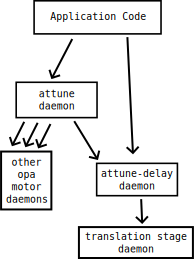
\includegraphics[width=5in]{active_correction/images/attune_delay_flow}
\caption[Attune Delay Information Flow]{The relationships between clients and daemons with an Attune Delay daemon.}
\label{act_corr:fig:attune_delay_flow}
\end{figure}

To make this work, the Attune Delay daemon exposes a set of messages that the light source Attune daemon can call to communicate changes.
Specifically, \texttt{set\_control\_tune} and \texttt{set\_control\_position} are called by the light source daemon at initialization and whenever the active arrangement or position, respectively, are changed.
When the Delay daemon receives these calls, it will recompute and reapply the offset.
The former accepts a string for the control key, i.e. the name of the light source daemon, and a string for the tune, which is the arrangement of the light source.
The latter similarly accepts the control key and a double precision floating point position.
Those are the only two messages that are used by the Attune daemon.

In addition, there are messages used by engineering interfaces or specialized clients to control the behavior of the Attune Delay daemon.
\texttt{set\_control\_active} allows for selectively turning off offsets from each light source.
This is useful for collecting the SDC offset curves themselves, which are typically collected without active correction applied to avoid needing to add two corrections together.
The position and tune caches are updated even if the controlling hardware is inactive.
This allows the correct offset to be applied if the hardware is toggled to active.
\texttt{set\_zero\_position} takes a position in the coordinates of the underlying translation stage and calls that position "zero" for the logical delay.
\texttt{set\_instrument} allows overwriting of the entire \texttt{Instrument} object.
This is used by data processing scripts to apply newly collected SDC curves.
The \texttt{Instrument} is stored in the Attune Store, where it can be reloaded.
Client connections are interrupted so that they are aware that assumptions about the applied \texttt{Instrument} are broken and they must refresh their cached copies.

Each of the setting methods mentioned above have associated methods for retrieving the information, as well as methods to get related quantities such as limits or units.

In all, the Attune Delay daemon looks just like any other \yaq{} daemon to a client program which does not require knowledge of the details of the offsetting behavior.
While all of the information is available to clients, if one wishes to do a simple one dimensional scan, it behaves just as any other motor.
Its only functional difference in that regard from the underlying translation stage is that the units and zero position are changed to represent the logical behavior of the stage as part of a larger instrument rather than the physical behavior of the stage alone.

\clearpage

\section{ndinterp}  % ===================================================================


Phase matching is an important factor contributing to the constructive interference of non-linear mixing processes. 
Some mixing processes cannot be phase matched, and therefore have destructive interference which causes diminished signal with increased path length.
To properly account for phase matching, relative angles of beam propagation combined with the energies and indices of refraction for each incident beam and the generated output beam must be taken into account.
Since it is wavelength dependent, a desired experiment may span a region where the optimal phase matching requires incoming light at significantly differing angles.
The Wright Group, and in particular Emily Kaufman, have been attempting to actively correct for angle of incidence to ensure proper phase matching for all wavelengths of a desired experiment.
To accomplish this task, the idea is to move the retroreflector laterally to displace the beam horizontally while maintaining the output angle from the retroreflector.
The beam will therefore hit a different position on the focusing optic.
The focussing optic will maintain focus for the parallel incoming beams to the same spot on the sample, but with differing angles.\footnote{This is technically only true for parabolic mirrors, but in practice is often a good enough approximation for spherical mirrors used approximately on axis}
Depending on the free aperture of the mirrors and the focal length of the focussing optic, this can provide several degrees of available offset while maintaining spatial overlap at the sample.
Figure \ref{act_corr:fig:phase_matching_angle} shows the effect of translating a retroreflector as described above.
This figure is not to scale, simply a cartoon illustrating the principle.
The ideal angle can be calculated, but is dependent on multiple laser colors in complicated ways.
Unlike SDC, phase matching corrections are not separable for each light source and additive.

\begin{figure}
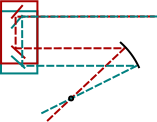
\includegraphics[width=5in]{active_correction/images/phase_matching_angle}
\caption[Phase Matching Angle]{The same incident beam angle will be translated if the retroreflector is translated.
A focussing optic causes the beams to converge to the same location in space but at different angles.}
\label{act_corr:fig:phase_matching_angle}
\end{figure}

The hardware required for active phase matching is a translation stage mounted perpendicular to the beam path with a retroreflector.
Because a retroreflector is already required for delays, this lateral translation stage is mounted on top of the delay
This does require some tight consideration for physical size of the translation stage, as it must both support the mass of the retroreflector and be short enough for mirrors to sit on top.

For this process, the information required is almost precisely the same as the Attune Delay daemon detailed above.
So, to accomplish the task, we must implement a daemon that looks to the light source Attune daemon exactly like an Attune Delay daemon.
This is not strictly required for this daemon specifically, but does allow it to be quickly implemented without changing existing daemons.
The daemon must be notified of when controlling hardware changes position and recompute its offsets.
This daemon, called NDInterp, performs N-Dimensional interpolation to be a maximally flexible active correction daemon.
However, the \texttt{Tune} information is not used, so a method which does nothing is provided so that the calling client daemon does not have to be changed. 
Instead of being backed by an Attune \texttt{Instrument} which accepts independent offsets which are additive, a single multidimensional offset is used.
This multidimensional offset is represented as a WrightTools Data file.
The data file is configured to have a single \texttt{WrightTools.Data} object which has axes of the control hardware and a channel which represents the required offset.
implement a daemon that looks to the opa exactly like an attune-delay
Similar to Attune Delay, NDInterp has a zero position from which all offsets are relative.

Since the offset is fundamentally multidimensional, independent control hardware cannot be toggled on and off like they can for the Delay daemon.
Instead, there is a single boolean \yaq{} property which can disable the offset behavior entirely to allow for experiments which do not require the active phase matching.

This approach to active phase matching allowed us to quickly and easily write a daemon that is capable of performing the active correction required.

\clearpage
  % act
%\chapter{WALDO: A case study on building a full instrument with \texttt{yaq}} \label{cha:waldo}

\clearpage

\section{Introduction}  % =========================================================================

\clearpage

\section{Design Requirements}  % =============================================================

\subsection{Specifications}

- rep rate
- pulse width
- number of tunable sources
- wavelength regions
- range for delay
- speed of detection, simultaneous acquisition


\subsection{Hardware Selection}

- many from same manufacturers as other systems
   - means yaq daemons are either done, or at least similar enough as to only require minimal perturbations
   - Extant Python interface a plus


\clearpage

\section{Implementing Daemons}  % ===================================================================

Much of the hardware comes before the core upstream laser is on the table
As hardware arrives, daemons can be created _before_ it goes on the table.
   - Some can be surmised from documentation, though it all must be tested thoroughly
   - yaq makes testing the interface easy, as there are limited, well documented, ways to interface with the hardware.
   - Mono had additional features: motorized mirrors and slits
   - Delays were a different model that had some initial bugs
   - Lightcon uses discrete motor positions

   New daemons:
   - Integrated array detector inside of one of the opas
   - gage daemon
      - Less able to be worked out before the system is assembled, as signals are key to ensuring correctness
      - Some done with pulse generators and such, but ultimately hard to fully replicate a running system.
      - discuss chopping

\clearpage

\section{Assemble the Instrument}  % ===================================================================

"The BIG day", when the upstream lasers get installed
   - Done by a tech
   - Can then build around it
      - Chopping
      - Optics for ensuring columation and beam size
      - delays
      - Focusing into sample
      - sample cell itself
      - focusing into mono
      - enclosure
      - alternate beam paths for tuning, etc
Bluesky + yaq = <3
   - Getting to experiments
   - Started with old setup
   - a false start or two with bluesky
Building custom instrument is never "final"
  - New ideas of new experiments to do
  - Temporary setups for short term experiments
     - Yoon group experiments
  - Future addt'l control of existing hardware
     - rep rate
     - chopping
     - upstream laser standby

Include photos and table

\begin{table}[]
\begin{tabular}{llllll}
\hline
host      & port  & kind                    & name               \\ \hline
127.0.0.1 & 39011 & thorlabs-bsc203         & d1\_stage          \\
127.0.0.1 & 39012 & thorlabs-bsc203         & d2\_stage          \\
127.0.0.1 & 38601 & lightcon-topas4-shutter & twin1\_shutter     \\
127.0.0.1 & 38602 & lightcon-topas4-shutter & twin2\_shutter     \\
127.0.0.1 & 38603 & lightcon-topas4-shutter & hp\_shutter        \\
127.0.0.1 & 38701 & lightcon-topas4-motor   & hp\_Delay\_1       \\
127.0.0.1 & 38702 & lightcon-topas4-motor   & hp\_Crystal\_1     \\
127.0.0.1 & 38703 & lightcon-topas4-motor   & hp\_Delay\_2       \\
127.0.0.1 & 38704 & lightcon-topas4-motor   & hp\_Crystal\_2     \\
127.0.0.1 & 38705 & lightcon-topas4-motor   & hp\_SHG\_Crystal   \\
127.0.0.1 & 38706 & lightcon-topas4-motor   & hp\_RP5\_Stage     \\
127.0.0.1 & 38707 & lightcon-topas4-motor   & hp\_WS\_Wheel\_1   \\
127.0.0.1 & 38708 & lightcon-topas4-motor   & hp\_RP6\_Stage     \\
127.0.0.1 & 38709 & lightcon-topas4-motor   & hp\_Crystal\_Stage\_2 \\
127.0.0.1 & 38710 & lightcon-topas4-motor   & hp\_WS\_Wheel\_2   \\
127.0.0.1 & 38801 & lightcon-topas4-motor   & twin1\_Delay_1     \\
127.0.0.1 & 38802 & lightcon-topas4-motor   & twin1\_Crystal\_1  \\
127.0.0.1 & 38803 & lightcon-topas4-motor   & twin1\_Delay\_2    \\
127.0.0.1 & 38804 & lightcon-topas4-motor   & twin1\_Crystal\_2  \\
127.0.0.1 & 38805 & lightcon-topas4-motor   & twin1\_RP\_Stage   \\
127.0.0.1 & 38806 & lightcon-topas4-motor   & twin1\_DFG\_CS\_1  \\
127.0.0.1 & 38901 & lightcon-topas4-motor   & twin2\_Delay\_1    \\
127.0.0.1 & 38902 & lightcon-topas4-motor   & twin2\_Crystal\_1  \\
127.0.0.1 & 38903 & lightcon-topas4-motor   & twin2\_Delay\_2    \\
127.0.0.1 & 38904 & lightcon-topas4-motor   & twin2\_Crystal\_2  \\
127.0.0.1 & 38905 & lightcon-topas4-motor   & twin2\_SHG\_Crystal \\
127.0.0.1 & 38906 & lightcon-topas4-motor   & twin2\_RP\_Stage   \\
127.0.0.1 & 38907 & lightcon-topas4-motor   & twin2\_DFG\_CS\_1  \\
127.0.0.1 & 38001 & attune                  & hp                 \\
127.0.0.1 & 38002 & attune                  & twin1              \\
127.0.0.1 & 38003 & attune                  & twin2              \\
127.0.0.1 & 39876 & horiba-ihr320           & mono               \\
127.0.0.1 & 39977 & rgb-qmini               & orpheus\_hp\_qmini \\
127.0.0.1 & 39001 & attune-delay            & d1                 \\
127.0.0.1 & 39002 & attune-delay            & d2                 \\
127.0.0.1 & 39003 & gage-compuscope         & daq                \\
127.0.0.1 & 38911 & thorlabs-pm-triggered   & thorlabs\_pm100d   \\
127.0.0.1 & 38401 & thorlabs-ell18          & hp\_FH\_IDL        \\
127.0.0.1 & 38500 & wright-fuyu-linear      & act                \\
127.0.0.1 & 38501 & wright-fuyu-linear      & pm1                \\
127.0.0.1 & 38502 & wright-fuyu-linear      & pm2                \\
127.0.0.1 & 38503 & wright-fuyu-linear      & pmtest             \\
127.0.0.1 & 36000 & system-monitor          & massive            \\
127.0.0.1 & 39200 & gdrive                  & gdrive             \\
127.0.0.1 & 38510 & newport-conex-agp       & filter1\_angle     \\
127.0.0.1 & 38010 & attune                  & filter1            \\ \hline
\end{tabular}
\caption[Waldo Daemons]{Summary of installed daemons on Waldo}
\label{waldo:tab:summary}
\end{table}


\clearpage


\part{Applications} \label{prt:applications}
\chapter{Active Correction as Daemons} \label{cha:act_corr}

\clearpage

\section{Introduction}  % =========================================================================

Blaise Thompson extensively discussed multiple forms of active corrections applied to CMDS instruments in Chapter 6 of his dissertation\cite{ThompsonBlaiseJonathan2018a}.
Most prominently, this includes Spectral Delay Correction (SDC).
At the time, active correction for SDC was performed by the orchestration layer, PyCMDS, as the ``autonomic'' system.
The implementation of the autonomic system was tightly coupled to the custom orchstration provided by PyCMDS.
This proved inflexible, and caused the hardware definitions to be intractable in many cases, leading to hard to understand behavior.

When the Wright Group was considering using Bluesky as an orchestration layer, the behavior of the autonomic system was one of the key pieces that made that transition seem hard at first.
There did not seem to be an easy and correct way of inserting the offset logic into the Bluesky Run Engine, as it was implemented for PyCMDS.
Additionally, Bluesky meant separating the behavior as collected, which runs through the Run Engine, from the behavior of hardware in an interactive session, as when attempting to initially find signal.
Upon reflecting, and taking a step back to consider the desired outcome, the solution became obvious: instead of inserting this logic as a modifier to the Run Engine, that logic can be implemented as a daemon which wraps the hardware daemon.
This intermediate daemon provides the controls of offsets being applied or ignored.
Additionally, daemons can be more specialized to the particular task, and thus are easier to use and describe compared to the general purpose autonomic system of PyCMDS.
To the client program, whether that is an interactive client like \yaqcqtpy{} or the Bluesky Run Engine, this daemon looks and acts like a simple motor that gets told to go to a particular position and does so.

Herein, we will look at two instances of active correction as daemons.
First, SDC itself and the \texttt{attune-delay} daemon which implements it.
And second, the \texttt{ndinterp} daemon which allows for more complicated relationships among controlling hardware.

\clearpage

\section{attune-delay}  % =============================================================

Spectral delay occurs largely due to transmissive optics which have a wavelength-dependent index of refraction and changes of the optical path length within the tunable light sources.
When pulses are less a picosecond long (or even shorter), even small variations will cause overlap in time to diminish rapidly.
Spectral Delay Correction (SDC) is an active correction technique which employs the delay motors already included in the instrument to adjust the path length of each beamline to account for any variation in arrival time as a function of wavelength.

SDC ``curves'' are represented as Attune \texttt{Instrument} objects.
This allows reuse of utilities that were used for OPA tuning curves previously.
For an OPA \texttt{Instrument} object, the whole thing represents one light source, each \texttt{Arrangement} represents one configuration of motors to produce a unique range of light, and each \texttt{Tune} represents the mapping of a single motor position (or another \texttt{Arrangement}) from the input color.
In contrast, for an SDC \texttt{Instrument} object, the levels are all shifted one down: the light source \texttt{Instrument} keys are the \texttt{Arrangement} keys of the SDC curve, and the \texttt{Arrangement} keys from the light sources are the \texttt{Tune} keys.
The \texttt{Tune} outputs are not motor positions directly, but rather offset in picoseconds for the particular light source using the particular \texttt{Arrangement}.
This allows a single \texttt{Instrument} to fully describe all possible required offsets for a laser system which may use multiple \texttt{Arrangement}s to do experiments.
The total offset is the sum of all offsets from each light source.

The objective is to create a daemon which performs the necessary offset.
Such a daemon will wrap a daemon for a translation stage, but can also perform the logical transform from displacement in length units to displacement in time units from some arbitrary zero mark which can be configured.
The offset will change whenever one of the values used to compute it changes: either a light source changes color or \texttt{Arrangement}.
When creating a daemon to compute and control the delay and offset, there is a natural inclination to have this daemon be a client of the light source and simply call for the color of the light source every time it computes the offset.
The problem with this is that the daemon has no way to tell that the color of a light source has changed.
To remedy this, a delay offset computing daemon would have to poll each light source for their position so that it could react as it needs to.
This tight polling is expensive, and requires balancing polling rate and responsiveness.
Additionally, when the light source changes color, it is possible that the delay will be the slowest motor, and so any client program will want the light source to remain busy until the associated delay is done moving.
All of these factors combined mean that instead, the Attune daemon which controls the light sources must be a client of the Attune Delay offsetting daemon.
The Attune Delay daemon simply caches the position and active arrangement of each controlling hardware and uses that cache to compute offsets.
It must recompute and reapply the offset whenever any controlling light source moves.
The Attune daemon can poll its associated delays for busy status whenever it moves, maintaining its own busy state that a client might be polling.
The client-daemon relationships are summarized in Figure \ref{act_corr:fig:attune_delay_flow}

\begin{figure}
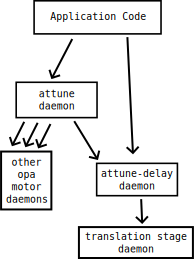
\includegraphics[width=5in]{active_correction/images/attune_delay_flow}
\caption[Attune Delay Information Flow]{The relationships between clients and daemons with an Attune Delay daemon.}
\label{act_corr:fig:attune_delay_flow}
\end{figure}

To make this work, the Attune Delay daemon exposes a set of messages that the light source Attune daemon can call to communicate changes.
Specifically, \texttt{set\_control\_tune} and \texttt{set\_control\_position} are called by the light source daemon at initialization and whenever the active arrangement or position, respectively, are changed.
When the Delay daemon receives these calls, it will recompute and reapply the offset.
The former accepts a string for the control key, i.e. the name of the light source daemon, and a string for the tune, which is the arrangement of the light source.
The latter similarly accepts the control key and a double precision floating point position.
Those are the only two messages that are used by the Attune daemon.

In addition, there are messages used by engineering interfaces or specialized clients to control the behavior of the Attune Delay daemon.
\texttt{set\_control\_active} allows for selectively turning off offsets from each light source.
This is useful for collecting the SDC offset curves themselves, which are typically collected without active correction applied to avoid needing to add two corrections together.
The position and tune caches are updated even if the controlling hardware is inactive.
This allows the correct offset to be applied if the hardware is toggled to active.
\texttt{set\_zero\_position} takes a position in the coordinates of the underlying translation stage and calls that position "zero" for the logical delay.
\texttt{set\_instrument} allows overwriting of the entire \texttt{Instrument} object.
This is used by data processing scripts to apply newly collected SDC curves.
The \texttt{Instrument} is stored in the Attune Store, where it can be reloaded.
Client connections are interrupted so that they are aware that assumptions about the applied \texttt{Instrument} are broken and they must refresh their cached copies.

Each of the setting methods mentioned above have associated methods for retrieving the information, as well as methods to get related quantities such as limits or units.

In all, the Attune Delay daemon looks just like any other \yaq{} daemon to a client program which does not require knowledge of the details of the offsetting behavior.
While all of the information is available to clients, if one wishes to do a simple one dimensional scan, it behaves just as any other motor.
Its only functional difference in that regard from the underlying translation stage is that the units and zero position are changed to represent the logical behavior of the stage as part of a larger instrument rather than the physical behavior of the stage alone.

\clearpage

\section{ndinterp}  % ===================================================================


Phase matching is an important factor contributing to the constructive interference of non-linear mixing processes. 
Some mixing processes cannot be phase matched, and therefore have destructive interference which causes diminished signal with increased path length.
To properly account for phase matching, relative angles of beam propagation combined with the energies and indices of refraction for each incident beam and the generated output beam must be taken into account.
Since it is wavelength dependent, a desired experiment may span a region where the optimal phase matching requires incoming light at significantly differing angles.
The Wright Group, and in particular Emily Kaufman, have been attempting to actively correct for angle of incidence to ensure proper phase matching for all wavelengths of a desired experiment.
To accomplish this task, the idea is to move the retroreflector laterally to displace the beam horizontally while maintaining the output angle from the retroreflector.
The beam will therefore hit a different position on the focusing optic.
The focussing optic will maintain focus for the parallel incoming beams to the same spot on the sample, but with differing angles.\footnote{This is technically only true for parabolic mirrors, but in practice is often a good enough approximation for spherical mirrors used approximately on axis}
Depending on the free aperture of the mirrors and the focal length of the focussing optic, this can provide several degrees of available offset while maintaining spatial overlap at the sample.
Figure \ref{act_corr:fig:phase_matching_angle} shows the effect of translating a retroreflector as described above.
This figure is not to scale, simply a cartoon illustrating the principle.
The ideal angle can be calculated, but is dependent on multiple laser colors in complicated ways.
Unlike SDC, phase matching corrections are not separable for each light source and additive.

\begin{figure}
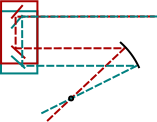
\includegraphics[width=5in]{active_correction/images/phase_matching_angle}
\caption[Phase Matching Angle]{The same incident beam angle will be translated if the retroreflector is translated.
A focussing optic causes the beams to converge to the same location in space but at different angles.}
\label{act_corr:fig:phase_matching_angle}
\end{figure}

The hardware required for active phase matching is a translation stage mounted perpendicular to the beam path with a retroreflector.
Because a retroreflector is already required for delays, this lateral translation stage is mounted on top of the delay
This does require some tight consideration for physical size of the translation stage, as it must both support the mass of the retroreflector and be short enough for mirrors to sit on top.

For this process, the information required is almost precisely the same as the Attune Delay daemon detailed above.
So, to accomplish the task, we must implement a daemon that looks to the light source Attune daemon exactly like an Attune Delay daemon.
This is not strictly required for this daemon specifically, but does allow it to be quickly implemented without changing existing daemons.
The daemon must be notified of when controlling hardware changes position and recompute its offsets.
This daemon, called NDInterp, performs N-Dimensional interpolation to be a maximally flexible active correction daemon.
However, the \texttt{Tune} information is not used, so a method which does nothing is provided so that the calling client daemon does not have to be changed. 
Instead of being backed by an Attune \texttt{Instrument} which accepts independent offsets which are additive, a single multidimensional offset is used.
This multidimensional offset is represented as a WrightTools Data file.
The data file is configured to have a single \texttt{WrightTools.Data} object which has axes of the control hardware and a channel which represents the required offset.
implement a daemon that looks to the opa exactly like an attune-delay
Similar to Attune Delay, NDInterp has a zero position from which all offsets are relative.

Since the offset is fundamentally multidimensional, independent control hardware cannot be toggled on and off like they can for the Delay daemon.
Instead, there is a single boolean \yaq{} property which can disable the offset behavior entirely to allow for experiments which do not require the active phase matching.

This approach to active phase matching allowed us to quickly and easily write a daemon that is capable of performing the active correction required.

\clearpage

\chapter{OPA400: A custom OPA built with \texttt{yaq}} \label{cha:opa400}

\clearpage

\section{Introduction}  % =========================================================================

An Optical Parametric Amplifier (OPA) is a device which allows for tunable control of the color of light produced.
In principle, a ``pump'' photon is split into two new photons, conventionally called ``signal'' and ``idler'' for the higher and lower energy photons, respectively.
The signal and idler photons observe conservation of energy, meaning that the sum of the two photon energies is equal to the pump photon energy.
The energy split is determined by a phase matching condition, which in our case is the angle with respect to the optical axis of a birefringent crystal, $\beta$-barium borate (BBO).
This process can be seeded by photons of the signal color, which increases efficiency of conversion.
To obtain this seed, an initial preamplification step is performed by using white light mixed with the pump laser in the birefringent crystal to produce a broad spectrum output.
This broad spectrum output is reflected off of a grating to select a narrow range of frequencies to be amplified using a second pass through the crystal.
Once signal and idler photons are created, additional mixing processes can be performed in additional crystals to produce new tunable wavelength ranges.
Commonly this includes doubling or even quadrupling the signal or idler photons, or adding in residual pump photons to either signal or idler.

For the picosecond laser system operated by the Wright Group, the upstream ``pump'' laser is 800 nm (12,500 $cm^{-1}$).
For OPAs pumped from this light, signal and idler are in the mid-infrared region, requiring additional mixing if visible light is desired.
What sets OPA400 apart from the other OPAs on the picosecond system is that rather than performing the additional mixing on the output photons, the pump laser is instead doubled to 400 nm (25,000 $cm^{-1}$) prior to splitting into signal and idler.
This means that the signal photons are themselves visible light between 750 nm and 450 nm, and the idler are correspondingly near infrared photons.
This provides a conveniently large tunable range in the visible light region with a single, smooth, tuning curve which avoids issues of needing to stitch together acquisitions from multiple tuning ranges.

\clearpage

\section{Design}  % =============================================================

The design of OPA400 encompasses both the optical components, the mechanical components used to control the photon split, and the driving electrical components for the mechanisms.
Many of the details of the design, including the custom electronic and mechanical parts, are available for this project 

\subsection{Optical Design}

The optical design of OPA400 mirrors closely the same principles of designing the laser table as a whole.
Optical path length is a critical dimension, so care must be taken when laying out optics and delay stages for fine adjustments are required.
The path lengths are folded for compact spatial design and having proper degrees of freedom for alignment.
High intensities are required for efficient generation of non-linear mixing, so focusing optics are required.
Overlap of multiple beams in the BBO crystal is crucial in both space and time.
Chromatically selective beam splitters are used pick off specific colors of light while allowing other colors, such as the parametric output, to pass through.
The layout of OPA400 is shown in schematic form in Figure \ref{opa4:fig:opa_schematic} and in photograph form in \ref{opa4:fig:opa_photo}.

\begin{figure}
	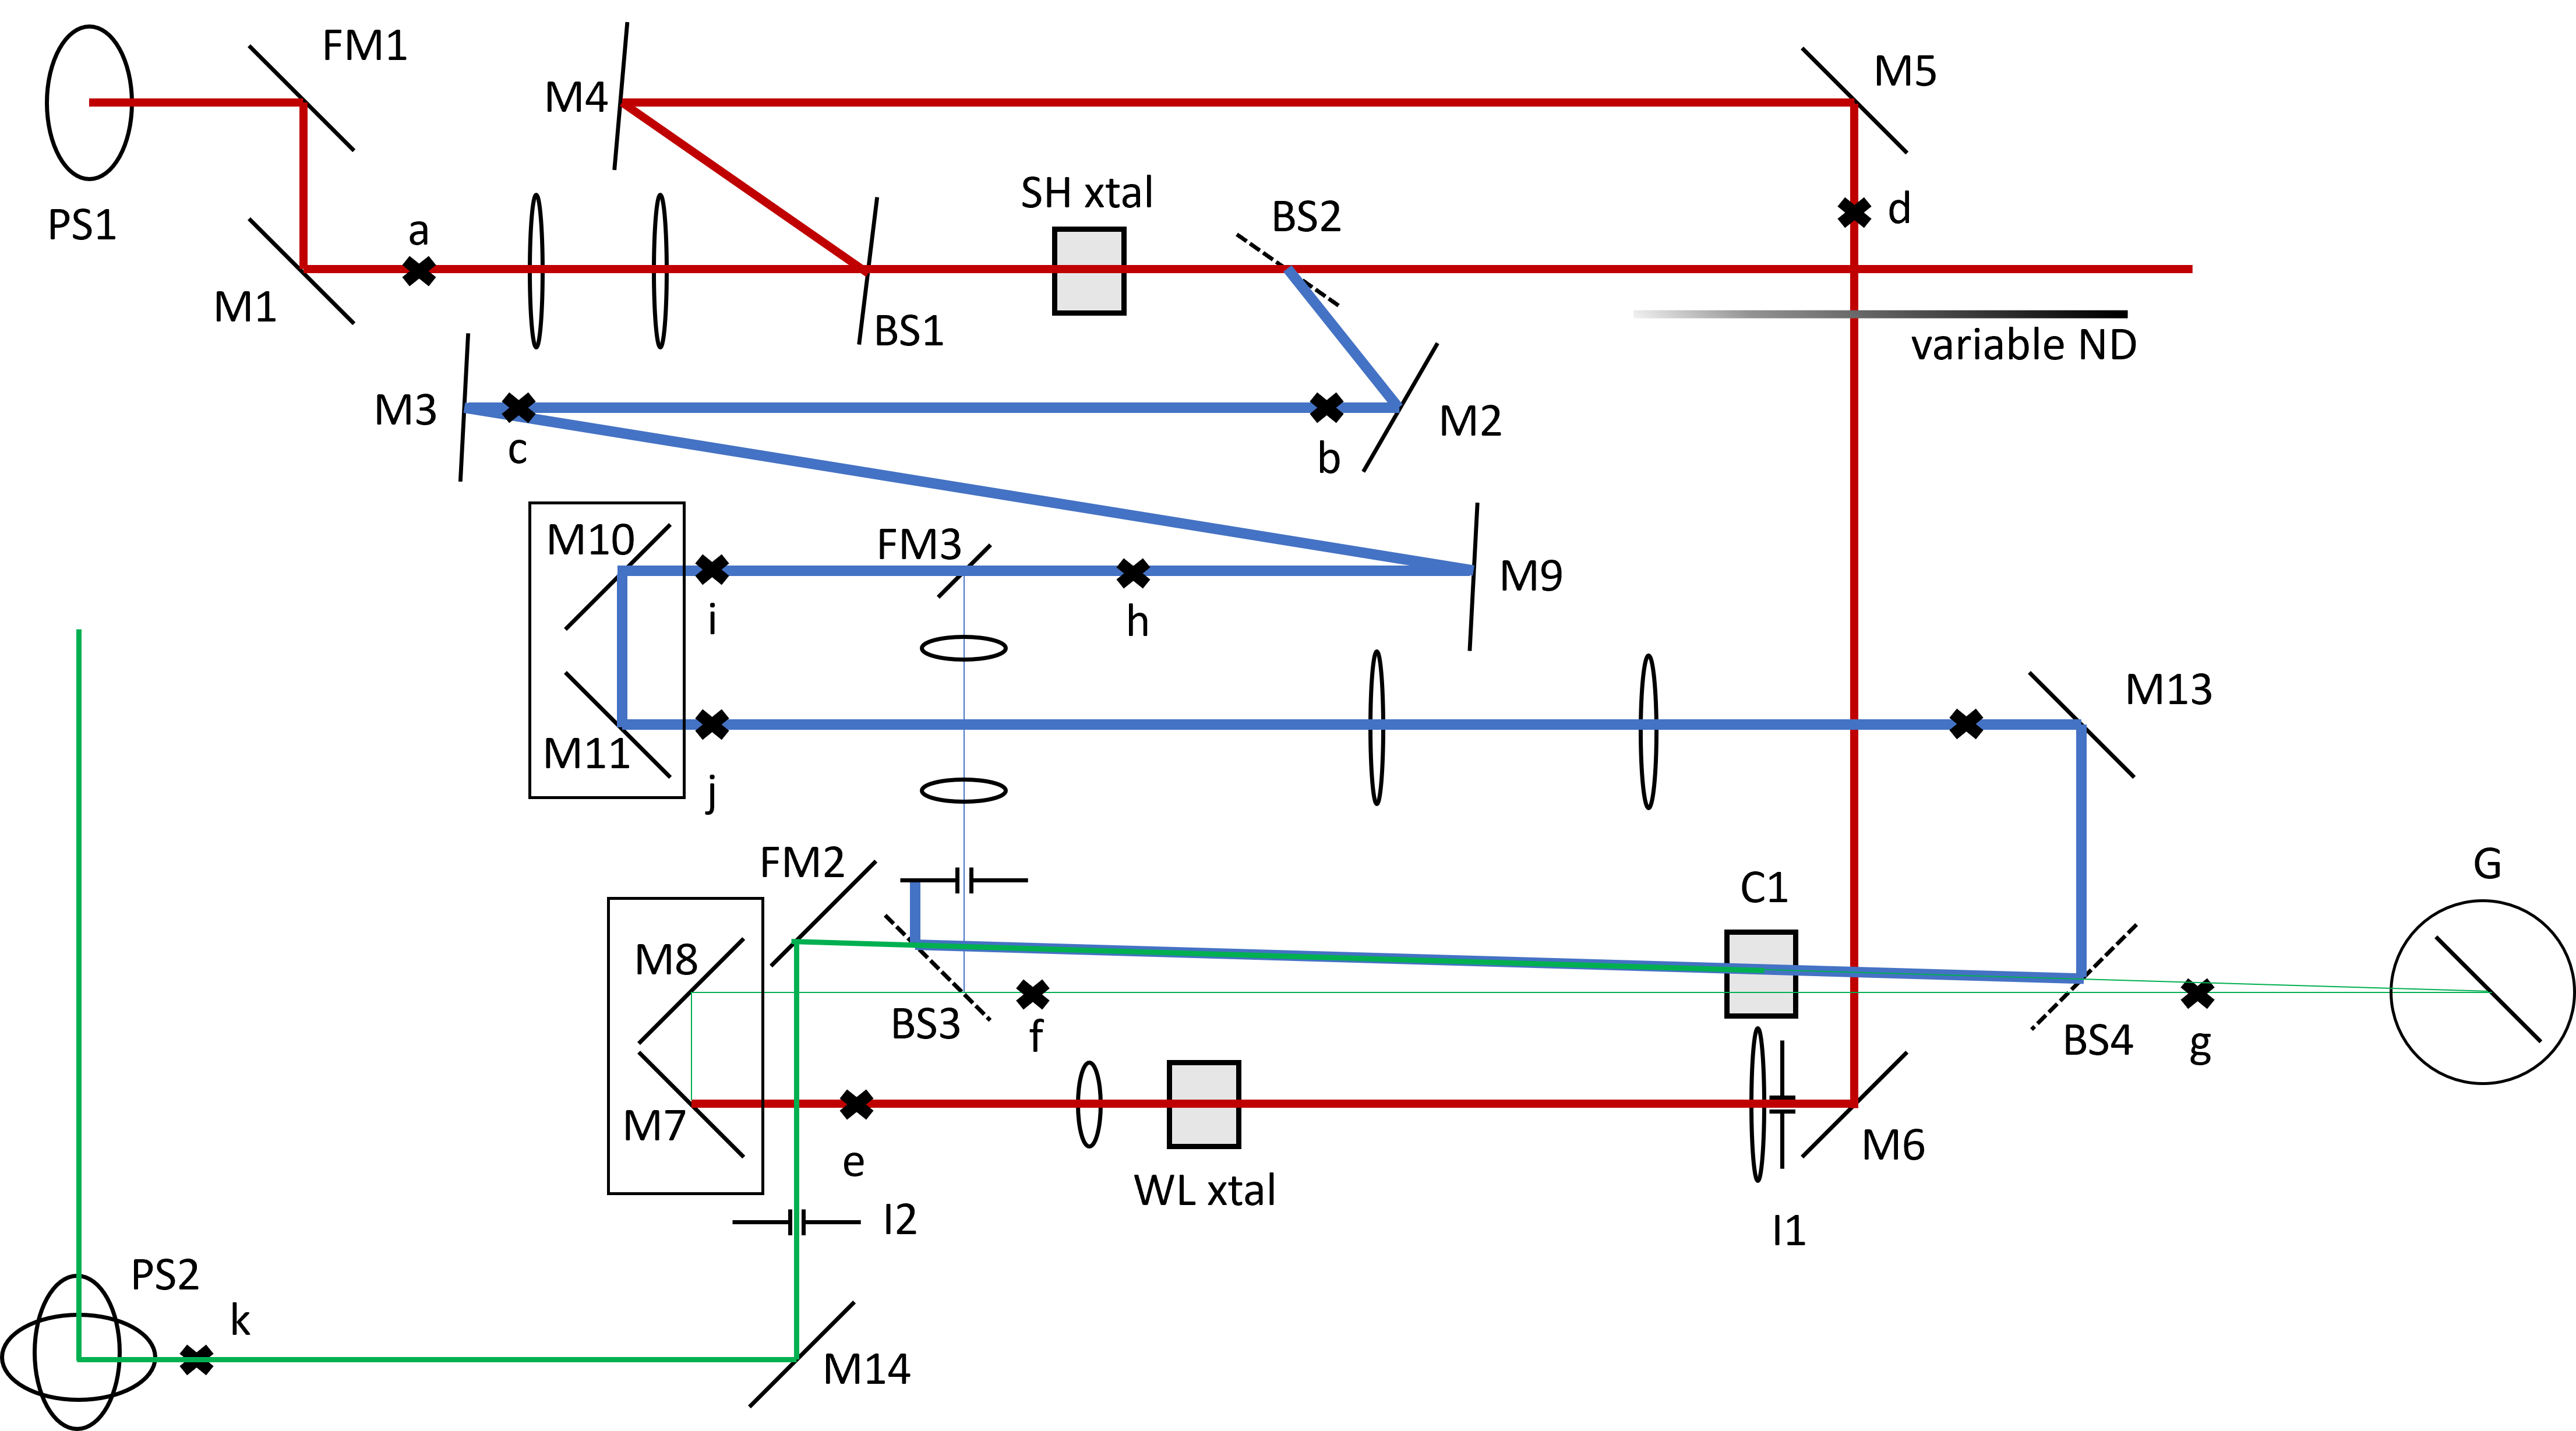
\includegraphics[width=6in]{opa400/images/opa400_schematic}
\caption[OPA 400 Optics]{
	Schematic view of OPA400.
	Input 800 nm light shown in red, doubled 400 nm light shown in blue, parametric output shown in green.
}
\label{opa4:fig:opa_schematic}
\end{figure}

\begin{figure}
	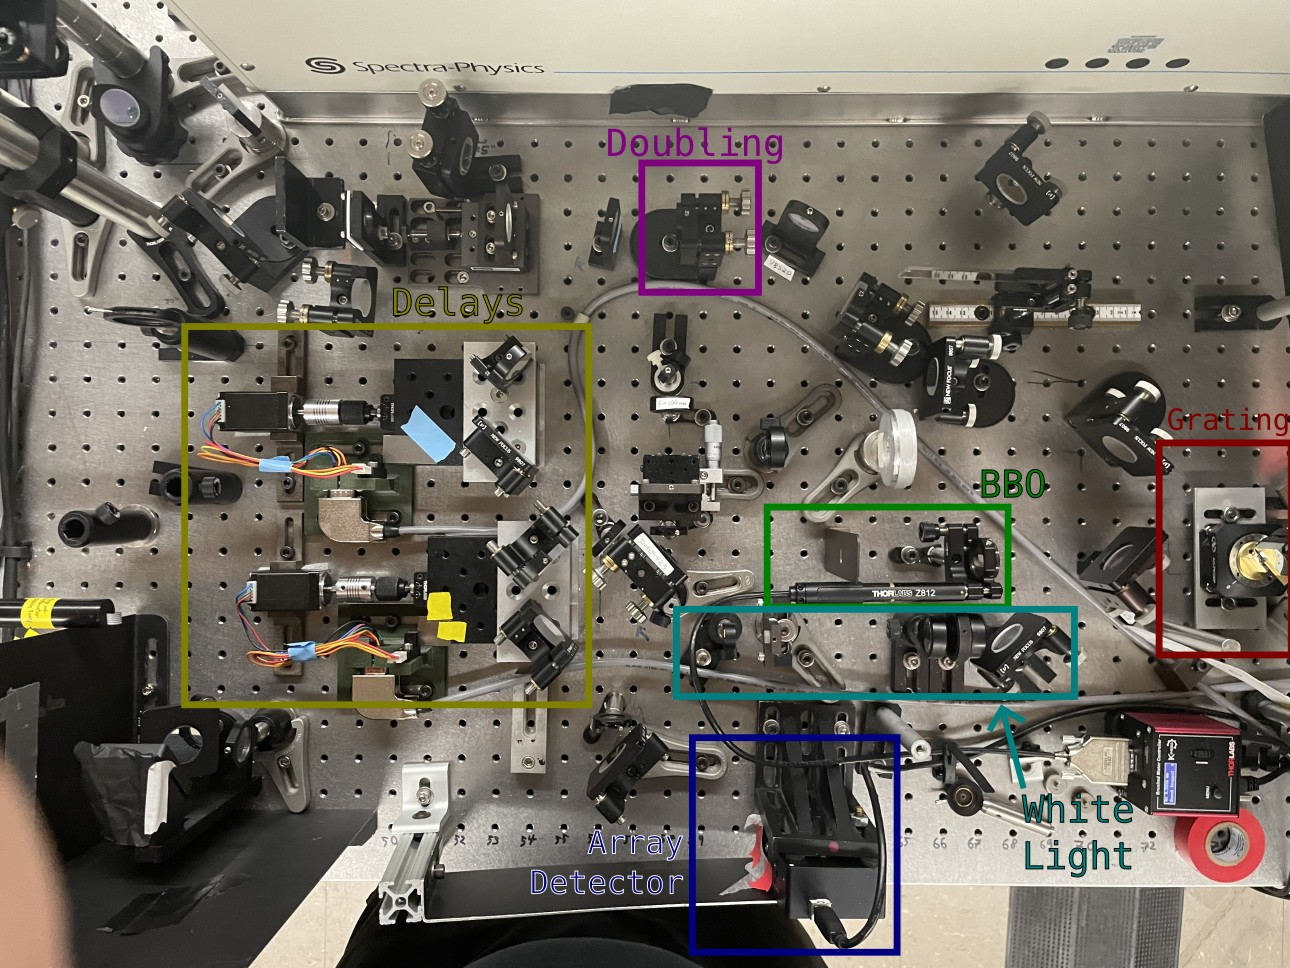
\includegraphics[width=6in]{opa400/images/opa400}
\caption[OPA 400 Optics]{
	Aerial view of OPA400. The 800 nm light enters at the top left and is doubled to 400 nm (purple). 
	A small portion of 800 nm light is used to generate white light (teal).
	The white light and a portion of the 400 nm pump light are combined initially in the BBO (green).
	This creates a broad spectrum output that is bounced off of the grating (red) back to the BBO (green).
	The delays (yellow) ensure that light arrives in the BBO at the same time, which is a requirement for mixing to occur.
	An array detector (blue) allows monitoring of the output visible signal photons.
}
\label{opa4:fig:opa_photo}
\end{figure}

\subsection{Hardware Selection}

The hardware selected follows a ``homebuilt'' approach.
Where possible, namely for the delay stages, standard NEMA stepper motors were used because they are cheap and highly available.
Where precision and/or compactness was a strict requirement, commercially available motors were used.
This includes the Thorlabs Z812\cite{thorlabs_z812} motor for controlling the angle of the BBO Crystal and the Newport CONEX-AGP\cite{newport_conex_agp} rotational mount for the grating.

Creating a complex component such as an OPA is an iterative process, with needs evolving as testing is performed.
For example, initially we opted not to include a grating, relying on phase matching angle alone for selectivity of the signal photon color.
This proved possible, but not as efficient or stable as we desired, so the grating was added as a revision.
The array detector, an Ocean Optics USB2000, is an optional but convenient addition which provides a tighter feedback loop when aligning the OPA.
Additionally, the original design used a Newport stepper motor to control the crystal angle.
The intent was to drive this motor with alternate stepper motor drivers.
This motor did not ultimately work as desired, so it was replaced with the Thorlabs motor and the associated manufacturer provided motor driver.

\clearpage
\section{Stepper Control Box}  % ===================================================================

The control system for this OPA centers around a Raspberry Pi 4\cite{rpi4}.
The stepper motors are driven by Adafruit Stepper Motor HATs\cite{adafruit_stepper_hat}.
These stepper motor drivers come in a convenient form of a circuit board that fits directly on top of the Raspberry Pi.
Each board can support two stepper motors, driven at a voltage provided to a power input that is not shared to the Raspberry Pi itself.
These boards can stack, allowing as many stepper motors as needed to be controlled from the same computer.

On top of the stepper motor driver boards, another hat is used to provide limit switch inputs.
This board is custom designed, containing eight digital inputs which accept 5 Volt input signal and provide a 3.3 Volt signal to the Raspberry Pi General Purpose Input Output (GPIO) pins.
The correspondence between input number as provided by the hat and digital GPIO pin used by the Raspberry Pi is provided in Table \ref{opa4:tab:interrupt_pinout}.
Each input has three pins associated with it: 5 Volts, Ground, and a signal pin.
The signal pin has a pull-up resistor for 5 Volts.
If a simple mechanical switch is used for the input, a nominally open switch between the signal and ground is sufficient.
The 5 Volt line is provided so that sensors such as optical interrupts which require power to operate can be used easily.
Figure \ref{opa4:fig:interrupt_schematic} shows a schematic representation of the schematic for the level conversion and LED indicator for a single input.
This motif is repeated eight times.
Figure \ref{opa4:fig:interrupt_board} shows a rendering of the circuit board itself.

\begin{table}[]                                                                                                     
\begin{tabular}{ll}                                                                                                 
\hline                                                                                                              
Interrupt Number & GPIO Pin   \\ \hline                                                                                        
1   & 17 \\                                                                                               
2   & 22 \\                                                                                               
3   & 5  \\                                                                                               
4   & 6  \\                                                                                               
5   & 13 \\                                                                                               
6   & 26 \\                                                                                               
7   & 23 \\                                                                                               
8   & 24 \\ \hline                                                                                        
\end{tabular}                                                                                                       
        \caption[Interrupt Hat GPIO Pins]{The pin correspondence the interrupt hat.}                         
        \label{opa4:tab:interrupt_pinout}                                                                                        
\end{table}     


\begin{figure}
	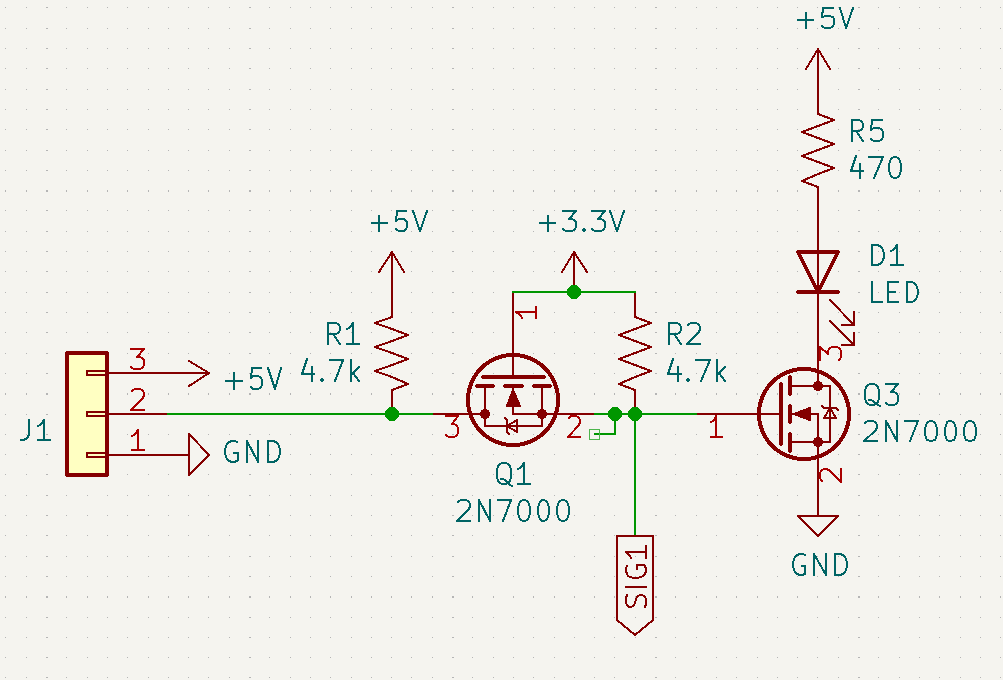
\includegraphics[width=5in]{opa400/images/interrupt_schematic}
\caption[Interrupt Hat Schematic]{
	A schematic view of a single input for the Interrupt Hat.
}
\label{opa4:fig:interrupt_schematic}
\end{figure}


\begin{figure}
	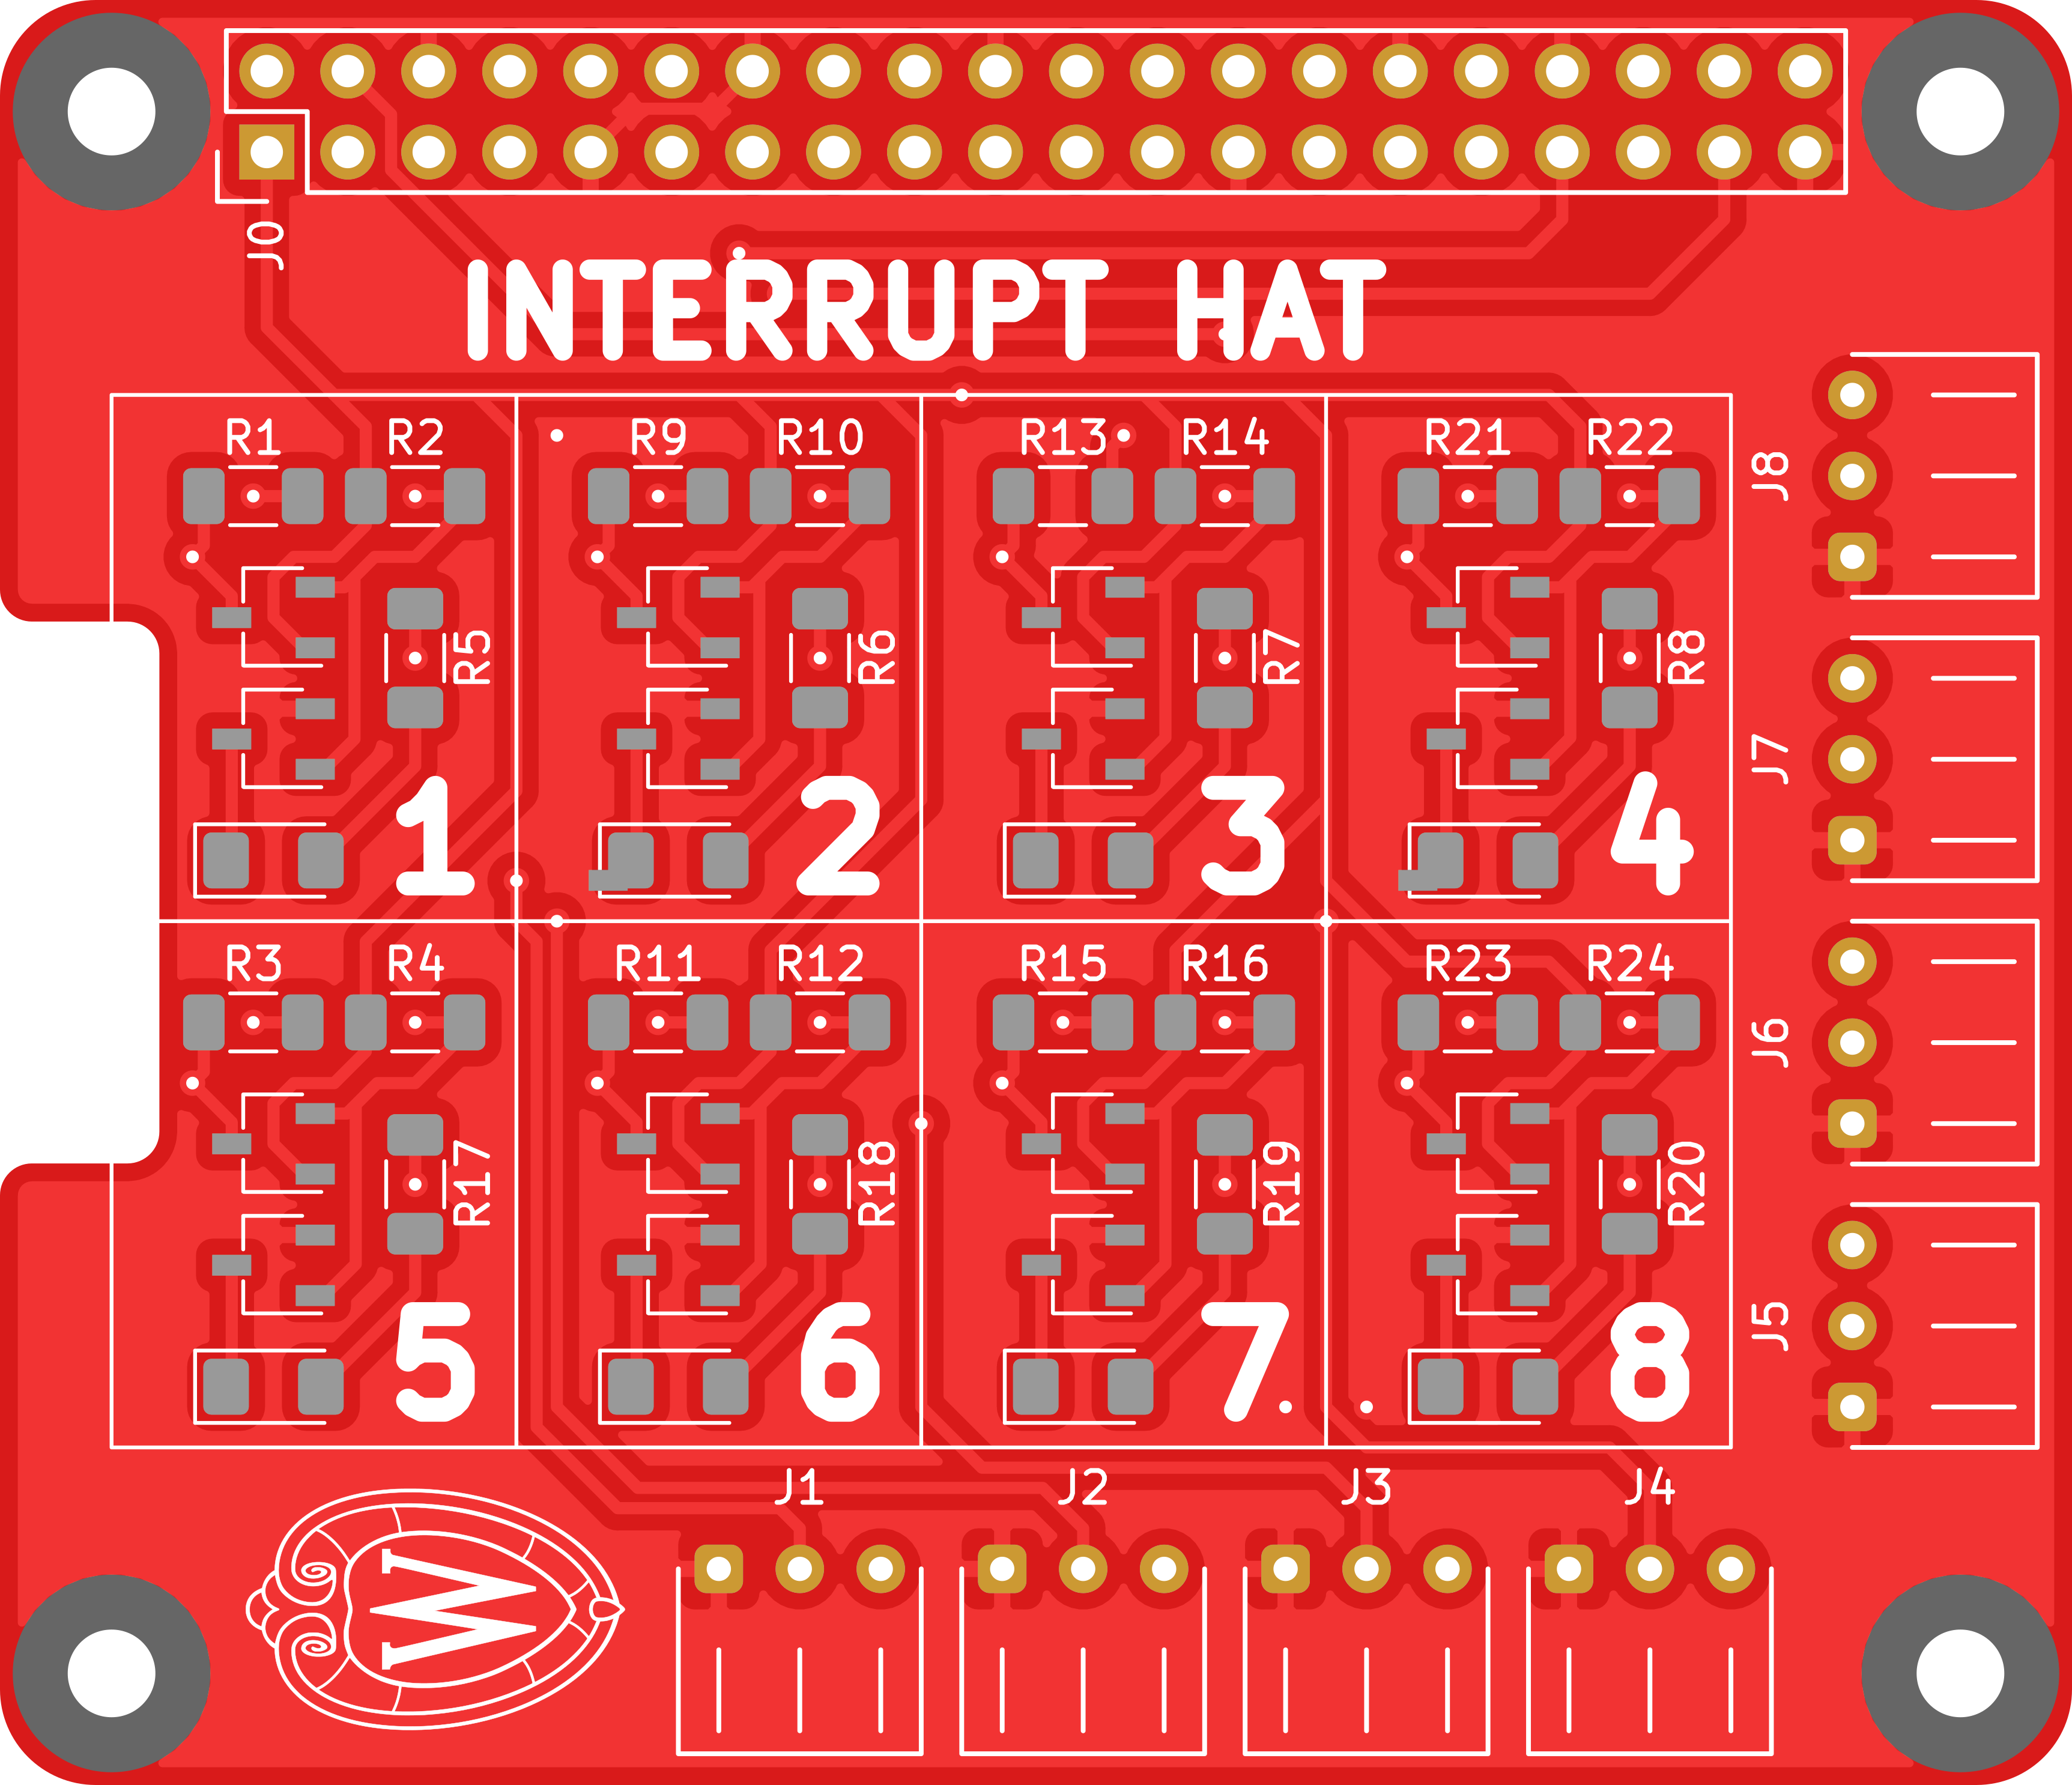
\includegraphics[width=4in]{opa400/images/interrupt_top}
	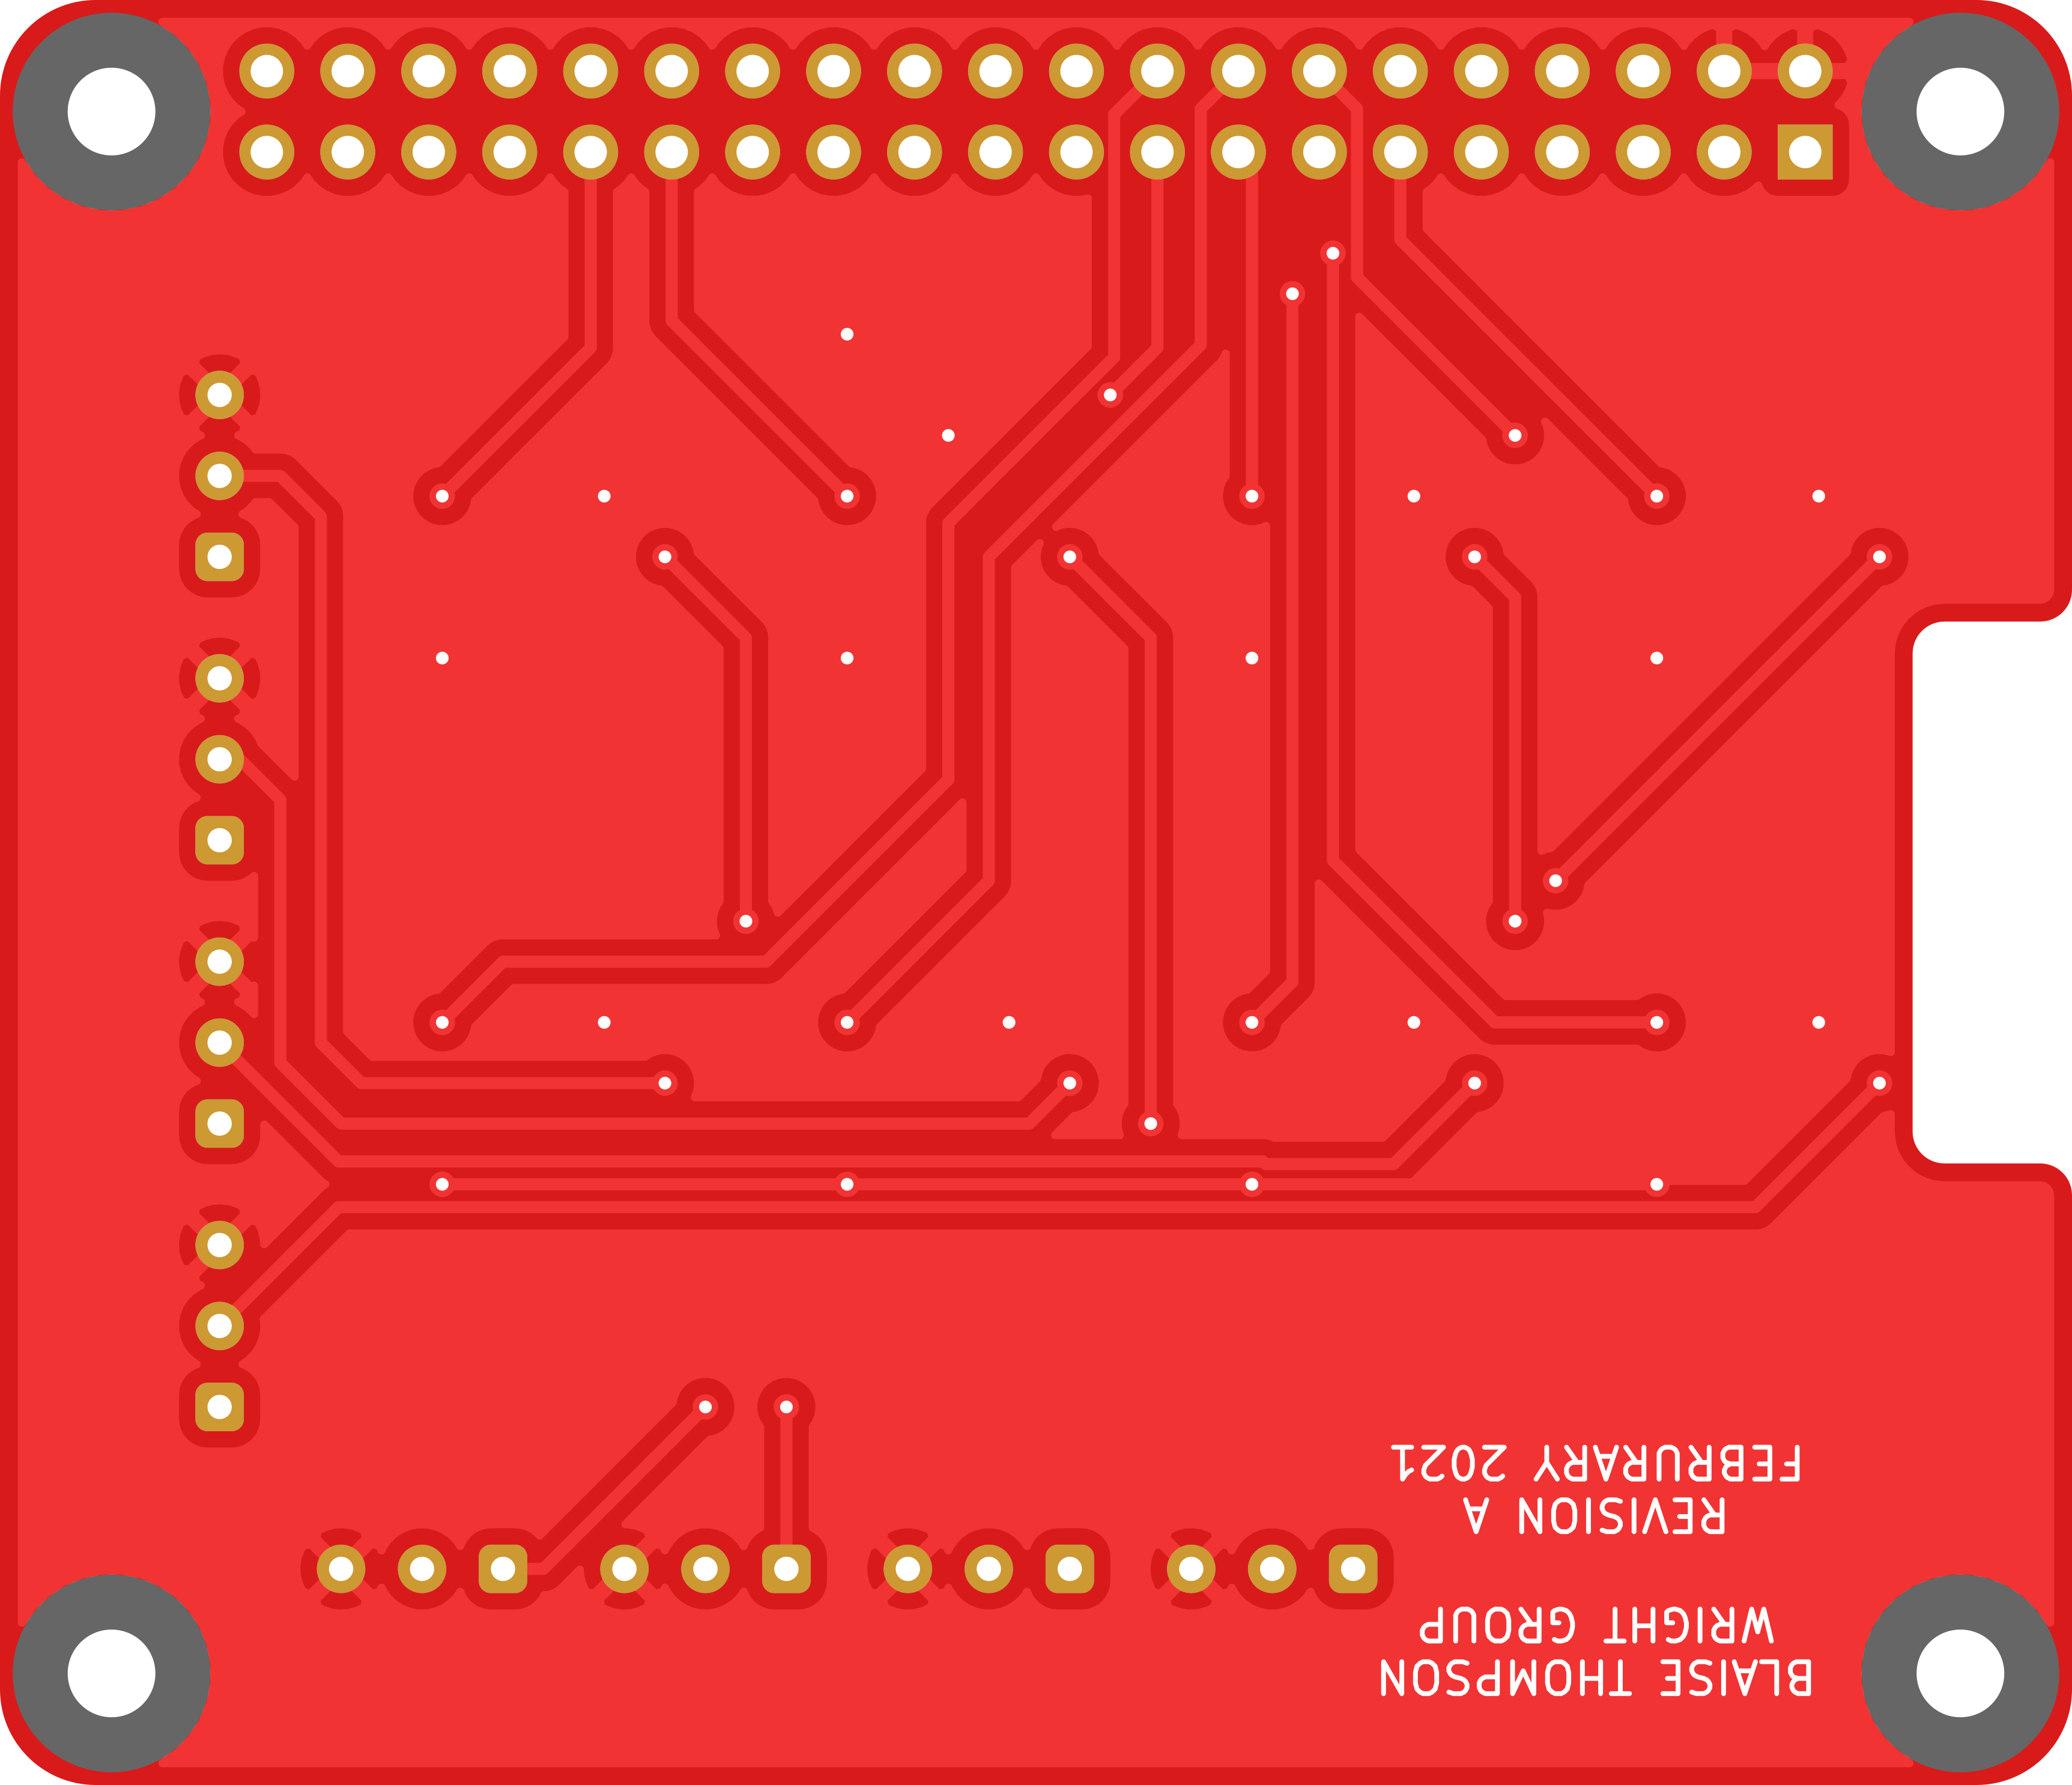
\includegraphics[width=4in]{opa400/images/interrupt_bottom}
\caption[Interrupt Hat Circuit Board]{
Rendering of the interrupt circuit board, top view and bottom view.
Rendering performed using tracespace\cite{tracespace}.
}
\label{opa4:fig:interrupt_board}
\end{figure}

The stepper control box is designed to work with the Mean Well RS-15 series of DC power supplies\cite{meanwell_rs15}.
Each hat level (two steppers) can accept an independent voltage level, so stepper motors with differing specifications can be used and controlled by the same system.
The box is designed so that three power supplies can be installed as needed.
One of the power supplies should be a 5 Volt power supply so that the Raspberry Pi itself can be powered from the same source.

The box is constructed of metal base with mounting holes drilled for the power supplies and the Raspberry Pi assembly.
At the corners of the base, 15 mm aluminum extrusion posts provide support for the panels.
The side panels and top are clear acrylic cut to size to slot in to the aluminum extrusion.
The top is secured with screws, with tapped 3 mm screw holes in the center of the posts.
This allows visual access to the LED indicators of the Interrupt Hat.
The front and rear panels are 3D printed plastic, with mounting for connectors.
The rear panel has AC power input and a power switch.
The front panel has a cut out for access to the Raspberry Pi USB and Ethernet ports as well as connectors for the stepper motors.
The pinout for the Wright Group's standard DE-9 D-subminiature stepper motor port is provided in Table \ref{opa4:tab:de9}.
Figure \ref{opa4:fig:control_box_photo} shows a photograph of the completed control box.

\begin{table}[]
\begin{tabular}{ll}
\hline
Pin & Connection   \\ \hline
1   & NC           \\
2   & Limit Signal \\
3   & +5 V         \\
4   & GND          \\
5   & NC           \\
6   & B2           \\
7   & B1           \\
8   & A1           \\
9   & A2           \\ \hline
\end{tabular}
	\caption[Stepper Motor DE9 Pinout]{The pinout for the stepper motor DE9 connector.}
	\label{opa4:tab:de9}
\end{table}

\begin{figure}
	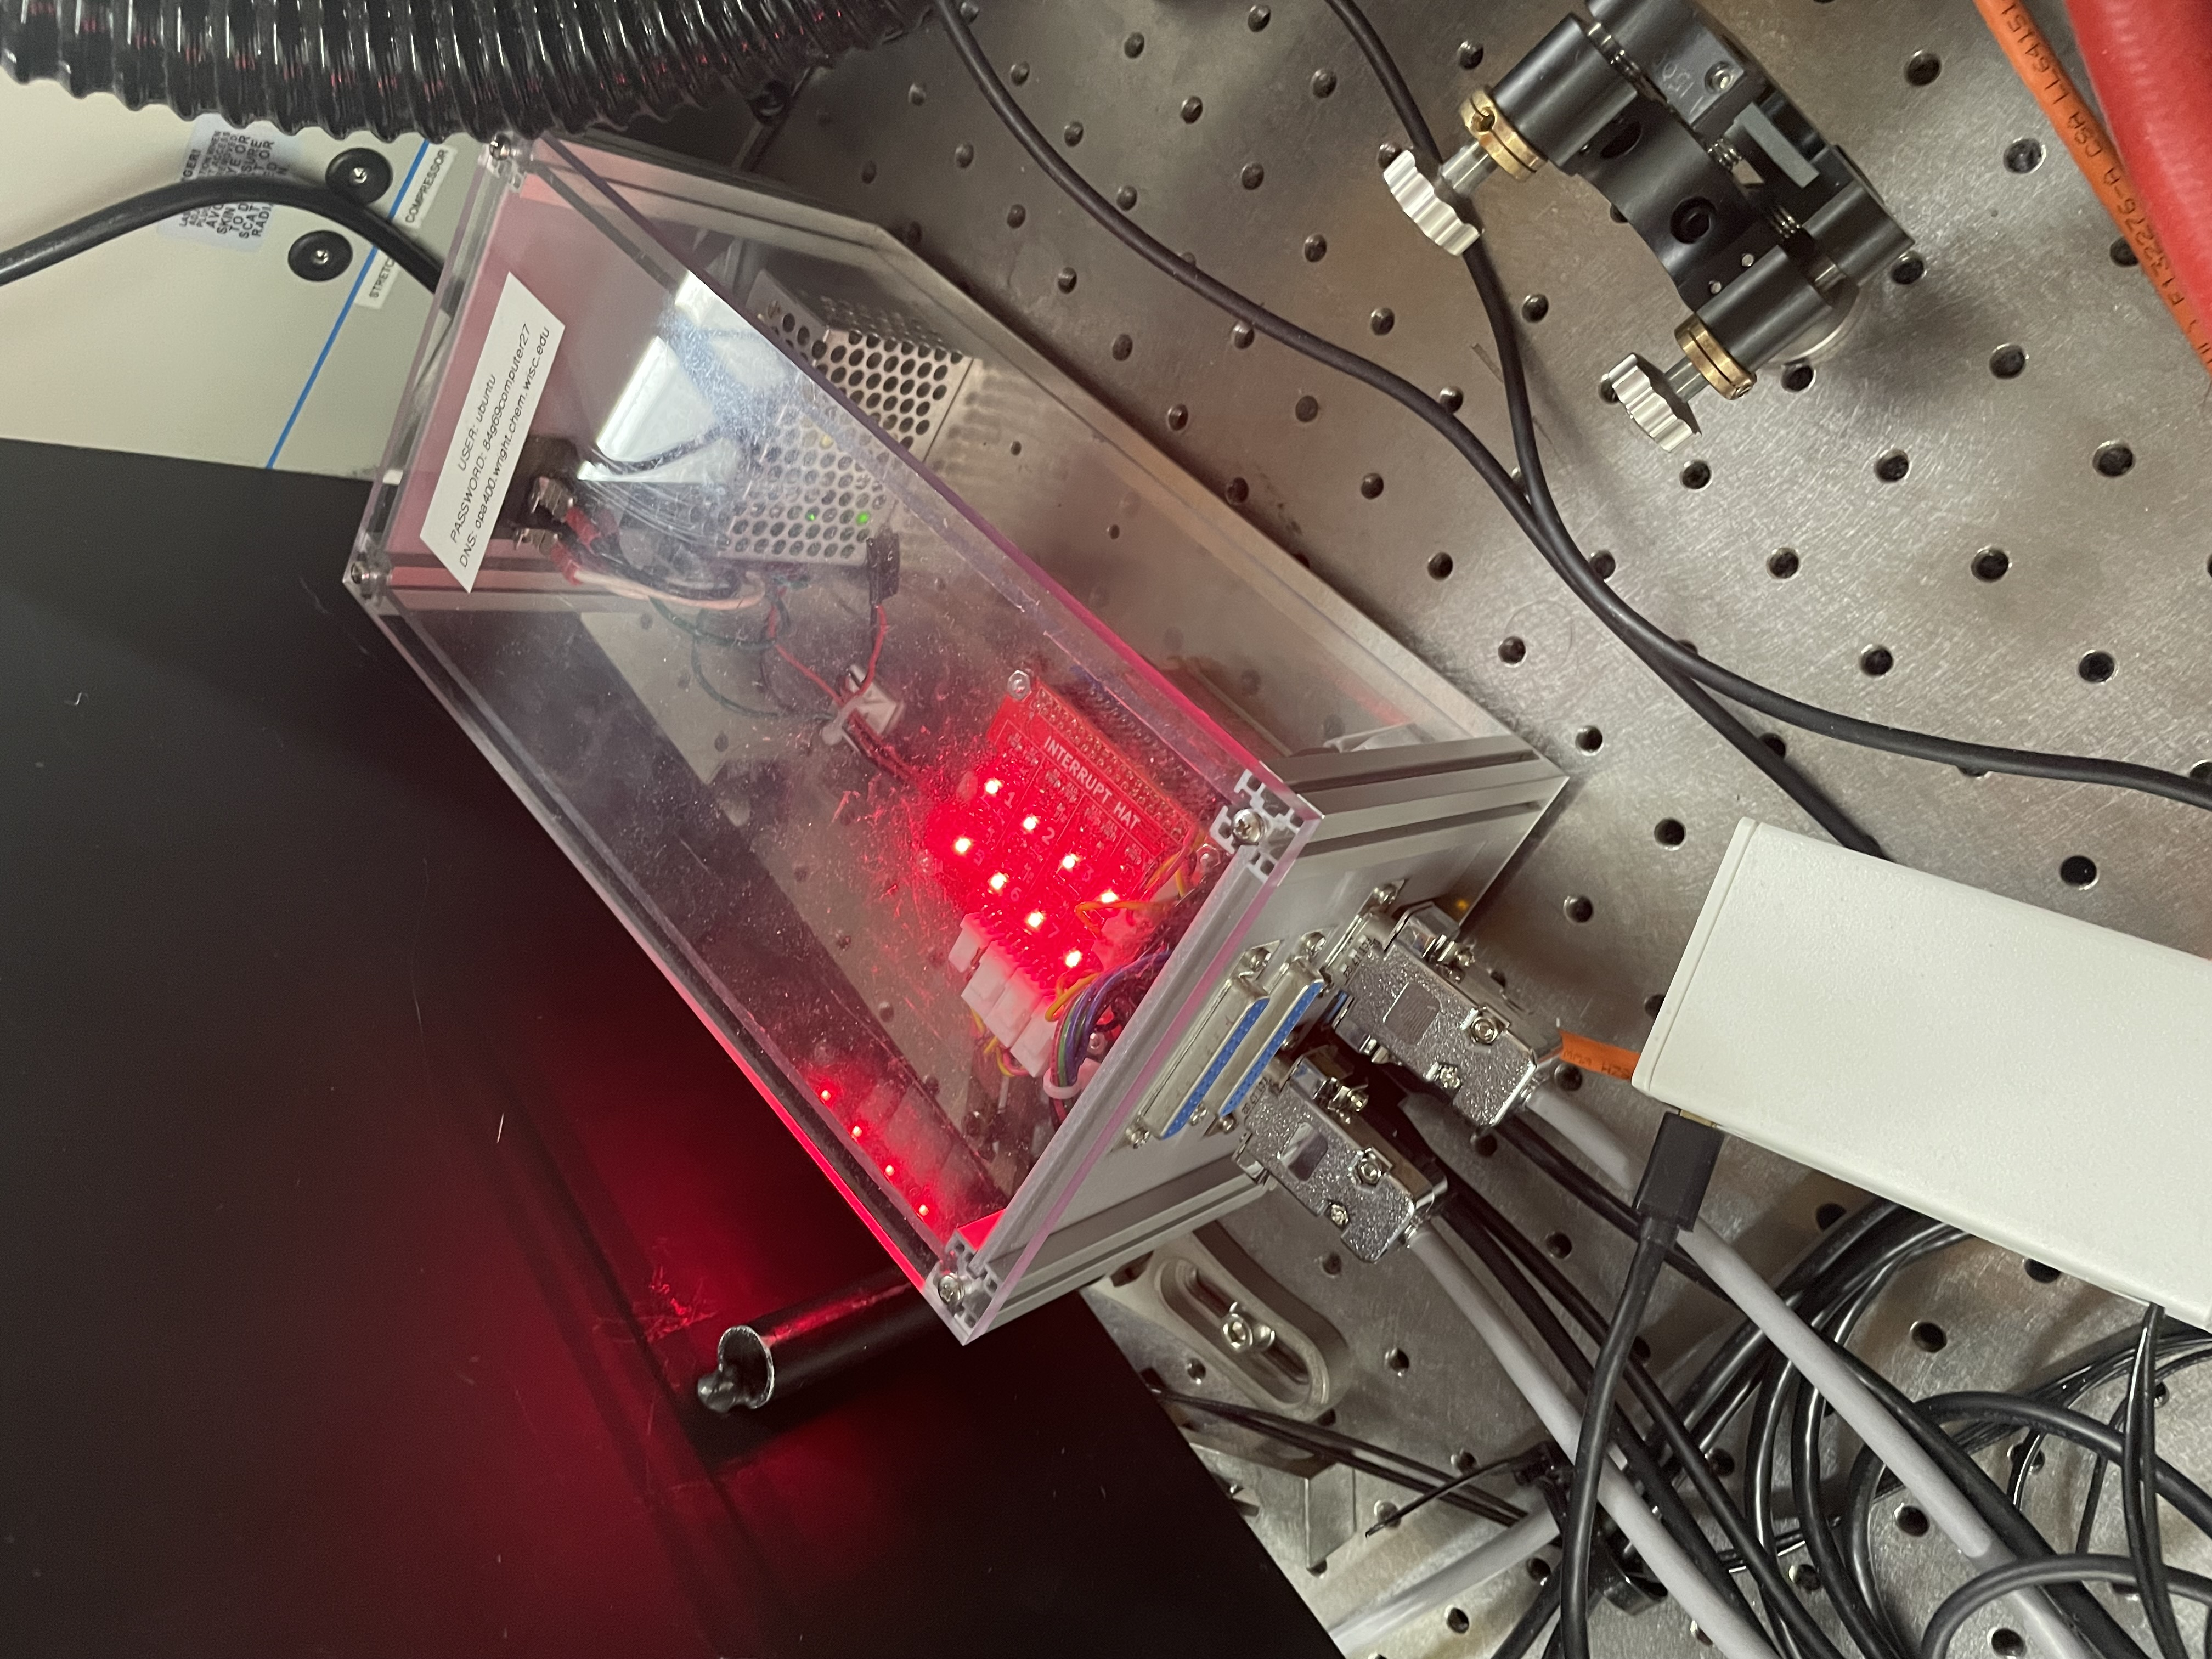
\includegraphics[width=5in]{opa400/images/opa400_control_box}
\caption[Stepper Control Box]{
Photograph of the stepper control box.
}
\label{opa4:fig:control_box_photo}
\end{figure}

\clearpage
\section{Delay stages}  % ===================================================================

The delay stages themselves have custom components designed for this application.
A 3D printed part provides a mount for a connector and the optical interrupt which is used for homing the motor.
A small piece of sheet metal is the flag which interrupts the optical interrupt.
The delay mechanism itself is a simple manual translation stage purchased from Thorlabs\cite{thorlabs_pt1b}.
This stage has a fine lead screw which provides the necessary precision to properly overlap the picosecond light pulses.
Below the stage, a machined aluminum block raises the stage to a height where the motor can directly drive the lead screw.
There is an additional adapter plate on top of the translation stage which provides a low profile mount for two mirrors at 90 degrees from each other, forming a planar retroreflector.
The custom machined parts in this system are important because space, particularly vertical space, is limited to have the mirrors in the desired position.
These parts were machined out of aluminum rather than 3D printed with consideration of the thermal expansion and rigidity of the parts which are directly supporting the optics.

The motors are coupled to the stage using a small aluminum rod machined to size and epoxied in place and a spring coupler which was purchased as a part for a 3D printer.
The motors themselves are mounted using two L-brackets pinching the motor.
Originally, the design included mounting the motor to the 3D printed part which also houses the connector and interrupt.
This proved problematic, as the forces exerted on the motor in the designed configuration meant it was unable to turn the stage.
Aligning the motor so that it can turn the stage is not difficult, but required more flexibility than a single mounting point of the 3D printed part.


\clearpage

\section{Software}  % ===================================================================

To control OPA400, a series of \yaq{} daemons were implemented.
Two of the motors were commercial products, the Thorlabs motor for the BBO crystal and the Newport motor for the grating.
These two had extant daemons already implemented prior to their use for OPA400\cite{yaqd-thorlabs}\cite{yaqd-newport}.
The Newport motor was already in use in other experimental setups, and had been written with the particular hardware that ended up installed in OPA400.
The Thorlabs motor was purchased specifically for this project, but uses a common protocol with other similar motors.
The daemon was already implemented, though it was tested specifically with the controller prior to installation.
These daemons can run directly on the Raspberry Pi, which makes for simpler cable management.

In addition to the previously created daemons, a new daemon was made to control the Adafruit stepper motor drivers.
This daemon uses two python libraries provided by Adafruit, the CircuitPython MotorKit\cite{adafruit-circuitpython-motorkit} and CircuitPython Motor\cite{adafruit-circuitpython-motor} libraries, as well as one library for interacting with the Raspberry Pi GPIO pins, GPIO Zero\cite{gpiozero}.
The first two are used to control the stepper motor, instructing each individual step.
The latter is used to read the state of the optical interrupt.
The daemon, implemented in about 100 lines of Python code, allows users to interact with the delay stages as they would with a daemon implemented for a commercial product.
Originally, this daemon was going to use another daemon for reading the interrupt state, but that was abandoned because of timing considerations and the fact that a daemon built for a Raspberry Pi hat is already a well constrained environment.
These daemons must be run directly on the Raspberry Pi, as they need direct hardware access to the GPIO pins.

Once each individual motor has an appropriate daemon implemented, the motors can be included in an Attune Instrument, just like other OPA models.
This Attune Instrument has its own daemon that can run on main instrument machine, which allows for easy access to update and read the Attune Instrument history.

When starting a new Attune Arrangement (or in this case a new Instrument altogether) a good initial strategy is to manually find appropriate motor positions for a small number of points.
Approximately five points, including points near to both ends of the expected usable range, is usually good enough to allow a general sense of the curvature of each Tune.
This rough tuning curve can be scaled up to more points (often around 20 points, though the degree of curvature and range will vary how many points are required for satisfactory interpolation) using \texttt{attune.map\_ind\_points}.
This upscaled Tune will not be fully accurate, but will usually be close enough that the standard tuning procedures can capture the offsets.

The standard tuning procedure for OPA400 is as follows.
First, a careful alignment of the optics, following standard operating procedures to align to apertures and obtain single color output.
Second a \texttt{run\_intensity} for the pre-amp delay (D1, the white light line) with the grating at normal incidence.
Third, a \texttt{run\_tune\_test} of the pre-amp color, using the array detector.
Fourth, a \texttt{run\_intensity} for the grating positions, detecting first pass amplification through an aperture.Finally, the second pass delay (D2, the delay for 400 nm light) is offset appropriately.
In theory, this delay needs to compensate for some additional spectral delay inside of the OPA.
In practice, a static offset is usually good enough for the whole range of colors.

\clearpage
  % opa 4 development case study
\chapter{WALDO: A case study on building a full instrument with \texttt{yaq}} \label{cha:waldo}

\clearpage

\section{Introduction}  % =========================================================================

\clearpage

\section{Design Requirements}  % =============================================================

\subsection{Specifications}

- rep rate
- pulse width
- number of tunable sources
- wavelength regions
- range for delay
- speed of detection, simultaneous acquisition


\subsection{Hardware Selection}

- many from same manufacturers as other systems
   - means yaq daemons are either done, or at least similar enough as to only require minimal perturbations
   - Extant Python interface a plus


\clearpage

\section{Implementing Daemons}  % ===================================================================

Much of the hardware comes before the core upstream laser is on the table
As hardware arrives, daemons can be created _before_ it goes on the table.
   - Some can be surmised from documentation, though it all must be tested thoroughly
   - yaq makes testing the interface easy, as there are limited, well documented, ways to interface with the hardware.
   - Mono had additional features: motorized mirrors and slits
   - Delays were a different model that had some initial bugs
   - Lightcon uses discrete motor positions

   New daemons:
   - Integrated array detector inside of one of the opas
   - gage daemon
      - Less able to be worked out before the system is assembled, as signals are key to ensuring correctness
      - Some done with pulse generators and such, but ultimately hard to fully replicate a running system.
      - discuss chopping

\clearpage

\section{Assemble the Instrument}  % ===================================================================

"The BIG day", when the upstream lasers get installed
   - Done by a tech
   - Can then build around it
      - Chopping
      - Optics for ensuring columation and beam size
      - delays
      - Focusing into sample
      - sample cell itself
      - focusing into mono
      - enclosure
      - alternate beam paths for tuning, etc
Bluesky + yaq = <3
   - Getting to experiments
   - Started with old setup
   - a false start or two with bluesky
Building custom instrument is never "final"
  - New ideas of new experiments to do
  - Temporary setups for short term experiments
     - Yoon group experiments
  - Future addt'l control of existing hardware
     - rep rate
     - chopping
     - upstream laser standby

Include photos and table

\begin{table}[]
\begin{tabular}{llllll}
\hline
host      & port  & kind                    & name               \\ \hline
127.0.0.1 & 39011 & thorlabs-bsc203         & d1\_stage          \\
127.0.0.1 & 39012 & thorlabs-bsc203         & d2\_stage          \\
127.0.0.1 & 38601 & lightcon-topas4-shutter & twin1\_shutter     \\
127.0.0.1 & 38602 & lightcon-topas4-shutter & twin2\_shutter     \\
127.0.0.1 & 38603 & lightcon-topas4-shutter & hp\_shutter        \\
127.0.0.1 & 38701 & lightcon-topas4-motor   & hp\_Delay\_1       \\
127.0.0.1 & 38702 & lightcon-topas4-motor   & hp\_Crystal\_1     \\
127.0.0.1 & 38703 & lightcon-topas4-motor   & hp\_Delay\_2       \\
127.0.0.1 & 38704 & lightcon-topas4-motor   & hp\_Crystal\_2     \\
127.0.0.1 & 38705 & lightcon-topas4-motor   & hp\_SHG\_Crystal   \\
127.0.0.1 & 38706 & lightcon-topas4-motor   & hp\_RP5\_Stage     \\
127.0.0.1 & 38707 & lightcon-topas4-motor   & hp\_WS\_Wheel\_1   \\
127.0.0.1 & 38708 & lightcon-topas4-motor   & hp\_RP6\_Stage     \\
127.0.0.1 & 38709 & lightcon-topas4-motor   & hp\_Crystal\_Stage\_2 \\
127.0.0.1 & 38710 & lightcon-topas4-motor   & hp\_WS\_Wheel\_2   \\
127.0.0.1 & 38801 & lightcon-topas4-motor   & twin1\_Delay_1     \\
127.0.0.1 & 38802 & lightcon-topas4-motor   & twin1\_Crystal\_1  \\
127.0.0.1 & 38803 & lightcon-topas4-motor   & twin1\_Delay\_2    \\
127.0.0.1 & 38804 & lightcon-topas4-motor   & twin1\_Crystal\_2  \\
127.0.0.1 & 38805 & lightcon-topas4-motor   & twin1\_RP\_Stage   \\
127.0.0.1 & 38806 & lightcon-topas4-motor   & twin1\_DFG\_CS\_1  \\
127.0.0.1 & 38901 & lightcon-topas4-motor   & twin2\_Delay\_1    \\
127.0.0.1 & 38902 & lightcon-topas4-motor   & twin2\_Crystal\_1  \\
127.0.0.1 & 38903 & lightcon-topas4-motor   & twin2\_Delay\_2    \\
127.0.0.1 & 38904 & lightcon-topas4-motor   & twin2\_Crystal\_2  \\
127.0.0.1 & 38905 & lightcon-topas4-motor   & twin2\_SHG\_Crystal \\
127.0.0.1 & 38906 & lightcon-topas4-motor   & twin2\_RP\_Stage   \\
127.0.0.1 & 38907 & lightcon-topas4-motor   & twin2\_DFG\_CS\_1  \\
127.0.0.1 & 38001 & attune                  & hp                 \\
127.0.0.1 & 38002 & attune                  & twin1              \\
127.0.0.1 & 38003 & attune                  & twin2              \\
127.0.0.1 & 39876 & horiba-ihr320           & mono               \\
127.0.0.1 & 39977 & rgb-qmini               & orpheus\_hp\_qmini \\
127.0.0.1 & 39001 & attune-delay            & d1                 \\
127.0.0.1 & 39002 & attune-delay            & d2                 \\
127.0.0.1 & 39003 & gage-compuscope         & daq                \\
127.0.0.1 & 38911 & thorlabs-pm-triggered   & thorlabs\_pm100d   \\
127.0.0.1 & 38401 & thorlabs-ell18          & hp\_FH\_IDL        \\
127.0.0.1 & 38500 & wright-fuyu-linear      & act                \\
127.0.0.1 & 38501 & wright-fuyu-linear      & pm1                \\
127.0.0.1 & 38502 & wright-fuyu-linear      & pm2                \\
127.0.0.1 & 38503 & wright-fuyu-linear      & pmtest             \\
127.0.0.1 & 36000 & system-monitor          & massive            \\
127.0.0.1 & 39200 & gdrive                  & gdrive             \\
127.0.0.1 & 38510 & newport-conex-agp       & filter1\_angle     \\
127.0.0.1 & 38010 & attune                  & filter1            \\ \hline
\end{tabular}
\caption[Waldo Daemons]{Summary of installed daemons on Waldo}
\label{waldo:tab:summary}
\end{table}


\clearpage


% appendix -----------------------------------------------------------------------------------------

\singlespacing

\part{Appendix} \label{prt:appendix}
\begin{appendix}
\chapter{Glossary} \label{cha:gloss}

\glsaddall
\printglossaries

\clearpage

%\chapter{Acquistion} \label{cha:acq}

\clearpage

\section{Introduction}  % =========================================================================

\clearpage

\section{Graphical user interface}  % =============================================================

\section{Internal structure}  % ===================================================================

\subsection{Multithreading}  % --------------------------------------------------------------------

\clearpage
  % prc
%\chapter{WALDO: A case study on building a full instrument with \texttt{yaq}} \label{cha:waldo}

\clearpage

\section{Introduction}  % =========================================================================

\clearpage

\section{Design Requirements}  % =============================================================

\subsection{Specifications}

- rep rate
- pulse width
- number of tunable sources
- wavelength regions
- range for delay
- speed of detection, simultaneous acquisition


\subsection{Hardware Selection}

- many from same manufacturers as other systems
   - means yaq daemons are either done, or at least similar enough as to only require minimal perturbations
   - Extant Python interface a plus


\clearpage

\section{Implementing Daemons}  % ===================================================================

Much of the hardware comes before the core upstream laser is on the table
As hardware arrives, daemons can be created _before_ it goes on the table.
   - Some can be surmised from documentation, though it all must be tested thoroughly
   - yaq makes testing the interface easy, as there are limited, well documented, ways to interface with the hardware.
   - Mono had additional features: motorized mirrors and slits
   - Delays were a different model that had some initial bugs
   - Lightcon uses discrete motor positions

   New daemons:
   - Integrated array detector inside of one of the opas
   - gage daemon
      - Less able to be worked out before the system is assembled, as signals are key to ensuring correctness
      - Some done with pulse generators and such, but ultimately hard to fully replicate a running system.
      - discuss chopping

\clearpage

\section{Assemble the Instrument}  % ===================================================================

"The BIG day", when the upstream lasers get installed
   - Done by a tech
   - Can then build around it
      - Chopping
      - Optics for ensuring columation and beam size
      - delays
      - Focusing into sample
      - sample cell itself
      - focusing into mono
      - enclosure
      - alternate beam paths for tuning, etc
Bluesky + yaq = <3
   - Getting to experiments
   - Started with old setup
   - a false start or two with bluesky
Building custom instrument is never "final"
  - New ideas of new experiments to do
  - Temporary setups for short term experiments
     - Yoon group experiments
  - Future addt'l control of existing hardware
     - rep rate
     - chopping
     - upstream laser standby

Include photos and table

\begin{table}[]
\begin{tabular}{llllll}
\hline
host      & port  & kind                    & name               \\ \hline
127.0.0.1 & 39011 & thorlabs-bsc203         & d1\_stage          \\
127.0.0.1 & 39012 & thorlabs-bsc203         & d2\_stage          \\
127.0.0.1 & 38601 & lightcon-topas4-shutter & twin1\_shutter     \\
127.0.0.1 & 38602 & lightcon-topas4-shutter & twin2\_shutter     \\
127.0.0.1 & 38603 & lightcon-topas4-shutter & hp\_shutter        \\
127.0.0.1 & 38701 & lightcon-topas4-motor   & hp\_Delay\_1       \\
127.0.0.1 & 38702 & lightcon-topas4-motor   & hp\_Crystal\_1     \\
127.0.0.1 & 38703 & lightcon-topas4-motor   & hp\_Delay\_2       \\
127.0.0.1 & 38704 & lightcon-topas4-motor   & hp\_Crystal\_2     \\
127.0.0.1 & 38705 & lightcon-topas4-motor   & hp\_SHG\_Crystal   \\
127.0.0.1 & 38706 & lightcon-topas4-motor   & hp\_RP5\_Stage     \\
127.0.0.1 & 38707 & lightcon-topas4-motor   & hp\_WS\_Wheel\_1   \\
127.0.0.1 & 38708 & lightcon-topas4-motor   & hp\_RP6\_Stage     \\
127.0.0.1 & 38709 & lightcon-topas4-motor   & hp\_Crystal\_Stage\_2 \\
127.0.0.1 & 38710 & lightcon-topas4-motor   & hp\_WS\_Wheel\_2   \\
127.0.0.1 & 38801 & lightcon-topas4-motor   & twin1\_Delay_1     \\
127.0.0.1 & 38802 & lightcon-topas4-motor   & twin1\_Crystal\_1  \\
127.0.0.1 & 38803 & lightcon-topas4-motor   & twin1\_Delay\_2    \\
127.0.0.1 & 38804 & lightcon-topas4-motor   & twin1\_Crystal\_2  \\
127.0.0.1 & 38805 & lightcon-topas4-motor   & twin1\_RP\_Stage   \\
127.0.0.1 & 38806 & lightcon-topas4-motor   & twin1\_DFG\_CS\_1  \\
127.0.0.1 & 38901 & lightcon-topas4-motor   & twin2\_Delay\_1    \\
127.0.0.1 & 38902 & lightcon-topas4-motor   & twin2\_Crystal\_1  \\
127.0.0.1 & 38903 & lightcon-topas4-motor   & twin2\_Delay\_2    \\
127.0.0.1 & 38904 & lightcon-topas4-motor   & twin2\_Crystal\_2  \\
127.0.0.1 & 38905 & lightcon-topas4-motor   & twin2\_SHG\_Crystal \\
127.0.0.1 & 38906 & lightcon-topas4-motor   & twin2\_RP\_Stage   \\
127.0.0.1 & 38907 & lightcon-topas4-motor   & twin2\_DFG\_CS\_1  \\
127.0.0.1 & 38001 & attune                  & hp                 \\
127.0.0.1 & 38002 & attune                  & twin1              \\
127.0.0.1 & 38003 & attune                  & twin2              \\
127.0.0.1 & 39876 & horiba-ihr320           & mono               \\
127.0.0.1 & 39977 & rgb-qmini               & orpheus\_hp\_qmini \\
127.0.0.1 & 39001 & attune-delay            & d1                 \\
127.0.0.1 & 39002 & attune-delay            & d2                 \\
127.0.0.1 & 39003 & gage-compuscope         & daq                \\
127.0.0.1 & 38911 & thorlabs-pm-triggered   & thorlabs\_pm100d   \\
127.0.0.1 & 38401 & thorlabs-ell18          & hp\_FH\_IDL        \\
127.0.0.1 & 38500 & wright-fuyu-linear      & act                \\
127.0.0.1 & 38501 & wright-fuyu-linear      & pm1                \\
127.0.0.1 & 38502 & wright-fuyu-linear      & pm2                \\
127.0.0.1 & 38503 & wright-fuyu-linear      & pmtest             \\
127.0.0.1 & 36000 & system-monitor          & massive            \\
127.0.0.1 & 39200 & gdrive                  & gdrive             \\
127.0.0.1 & 38510 & newport-conex-agp       & filter1\_angle     \\
127.0.0.1 & 38010 & attune                  & filter1            \\ \hline
\end{tabular}
\caption[Waldo Daemons]{Summary of installed daemons on Waldo}
\label{waldo:tab:summary}
\end{table}


\clearpage
  % irf
%\chapter{WALDO: A case study on building a full instrument with \texttt{yaq}} \label{cha:waldo}

\clearpage

\section{Introduction}  % =========================================================================

\clearpage

\section{Design Requirements}  % =============================================================

\subsection{Specifications}

- rep rate
- pulse width
- number of tunable sources
- wavelength regions
- range for delay
- speed of detection, simultaneous acquisition


\subsection{Hardware Selection}

- many from same manufacturers as other systems
   - means yaq daemons are either done, or at least similar enough as to only require minimal perturbations
   - Extant Python interface a plus


\clearpage

\section{Implementing Daemons}  % ===================================================================

Much of the hardware comes before the core upstream laser is on the table
As hardware arrives, daemons can be created _before_ it goes on the table.
   - Some can be surmised from documentation, though it all must be tested thoroughly
   - yaq makes testing the interface easy, as there are limited, well documented, ways to interface with the hardware.
   - Mono had additional features: motorized mirrors and slits
   - Delays were a different model that had some initial bugs
   - Lightcon uses discrete motor positions

   New daemons:
   - Integrated array detector inside of one of the opas
   - gage daemon
      - Less able to be worked out before the system is assembled, as signals are key to ensuring correctness
      - Some done with pulse generators and such, but ultimately hard to fully replicate a running system.
      - discuss chopping

\clearpage

\section{Assemble the Instrument}  % ===================================================================

"The BIG day", when the upstream lasers get installed
   - Done by a tech
   - Can then build around it
      - Chopping
      - Optics for ensuring columation and beam size
      - delays
      - Focusing into sample
      - sample cell itself
      - focusing into mono
      - enclosure
      - alternate beam paths for tuning, etc
Bluesky + yaq = <3
   - Getting to experiments
   - Started with old setup
   - a false start or two with bluesky
Building custom instrument is never "final"
  - New ideas of new experiments to do
  - Temporary setups for short term experiments
     - Yoon group experiments
  - Future addt'l control of existing hardware
     - rep rate
     - chopping
     - upstream laser standby

Include photos and table

\begin{table}[]
\begin{tabular}{llllll}
\hline
host      & port  & kind                    & name               \\ \hline
127.0.0.1 & 39011 & thorlabs-bsc203         & d1\_stage          \\
127.0.0.1 & 39012 & thorlabs-bsc203         & d2\_stage          \\
127.0.0.1 & 38601 & lightcon-topas4-shutter & twin1\_shutter     \\
127.0.0.1 & 38602 & lightcon-topas4-shutter & twin2\_shutter     \\
127.0.0.1 & 38603 & lightcon-topas4-shutter & hp\_shutter        \\
127.0.0.1 & 38701 & lightcon-topas4-motor   & hp\_Delay\_1       \\
127.0.0.1 & 38702 & lightcon-topas4-motor   & hp\_Crystal\_1     \\
127.0.0.1 & 38703 & lightcon-topas4-motor   & hp\_Delay\_2       \\
127.0.0.1 & 38704 & lightcon-topas4-motor   & hp\_Crystal\_2     \\
127.0.0.1 & 38705 & lightcon-topas4-motor   & hp\_SHG\_Crystal   \\
127.0.0.1 & 38706 & lightcon-topas4-motor   & hp\_RP5\_Stage     \\
127.0.0.1 & 38707 & lightcon-topas4-motor   & hp\_WS\_Wheel\_1   \\
127.0.0.1 & 38708 & lightcon-topas4-motor   & hp\_RP6\_Stage     \\
127.0.0.1 & 38709 & lightcon-topas4-motor   & hp\_Crystal\_Stage\_2 \\
127.0.0.1 & 38710 & lightcon-topas4-motor   & hp\_WS\_Wheel\_2   \\
127.0.0.1 & 38801 & lightcon-topas4-motor   & twin1\_Delay_1     \\
127.0.0.1 & 38802 & lightcon-topas4-motor   & twin1\_Crystal\_1  \\
127.0.0.1 & 38803 & lightcon-topas4-motor   & twin1\_Delay\_2    \\
127.0.0.1 & 38804 & lightcon-topas4-motor   & twin1\_Crystal\_2  \\
127.0.0.1 & 38805 & lightcon-topas4-motor   & twin1\_RP\_Stage   \\
127.0.0.1 & 38806 & lightcon-topas4-motor   & twin1\_DFG\_CS\_1  \\
127.0.0.1 & 38901 & lightcon-topas4-motor   & twin2\_Delay\_1    \\
127.0.0.1 & 38902 & lightcon-topas4-motor   & twin2\_Crystal\_1  \\
127.0.0.1 & 38903 & lightcon-topas4-motor   & twin2\_Delay\_2    \\
127.0.0.1 & 38904 & lightcon-topas4-motor   & twin2\_Crystal\_2  \\
127.0.0.1 & 38905 & lightcon-topas4-motor   & twin2\_SHG\_Crystal \\
127.0.0.1 & 38906 & lightcon-topas4-motor   & twin2\_RP\_Stage   \\
127.0.0.1 & 38907 & lightcon-topas4-motor   & twin2\_DFG\_CS\_1  \\
127.0.0.1 & 38001 & attune                  & hp                 \\
127.0.0.1 & 38002 & attune                  & twin1              \\
127.0.0.1 & 38003 & attune                  & twin2              \\
127.0.0.1 & 39876 & horiba-ihr320           & mono               \\
127.0.0.1 & 39977 & rgb-qmini               & orpheus\_hp\_qmini \\
127.0.0.1 & 39001 & attune-delay            & d1                 \\
127.0.0.1 & 39002 & attune-delay            & d2                 \\
127.0.0.1 & 39003 & gage-compuscope         & daq                \\
127.0.0.1 & 38911 & thorlabs-pm-triggered   & thorlabs\_pm100d   \\
127.0.0.1 & 38401 & thorlabs-ell18          & hp\_FH\_IDL        \\
127.0.0.1 & 38500 & wright-fuyu-linear      & act                \\
127.0.0.1 & 38501 & wright-fuyu-linear      & pm1                \\
127.0.0.1 & 38502 & wright-fuyu-linear      & pm2                \\
127.0.0.1 & 38503 & wright-fuyu-linear      & pmtest             \\
127.0.0.1 & 36000 & system-monitor          & massive            \\
127.0.0.1 & 39200 & gdrive                  & gdrive             \\
127.0.0.1 & 38510 & newport-conex-agp       & filter1\_angle     \\
127.0.0.1 & 38010 & attune                  & filter1            \\ \hline
\end{tabular}
\caption[Waldo Daemons]{Summary of installed daemons on Waldo}
\label{waldo:tab:summary}
\end{table}


\clearpage
  % qta
%\chapter{WALDO: A case study on building a full instrument with \texttt{yaq}} \label{cha:waldo}

\clearpage

\section{Introduction}  % =========================================================================

\clearpage

\section{Design Requirements}  % =============================================================

\subsection{Specifications}

- rep rate
- pulse width
- number of tunable sources
- wavelength regions
- range for delay
- speed of detection, simultaneous acquisition


\subsection{Hardware Selection}

- many from same manufacturers as other systems
   - means yaq daemons are either done, or at least similar enough as to only require minimal perturbations
   - Extant Python interface a plus


\clearpage

\section{Implementing Daemons}  % ===================================================================

Much of the hardware comes before the core upstream laser is on the table
As hardware arrives, daemons can be created _before_ it goes on the table.
   - Some can be surmised from documentation, though it all must be tested thoroughly
   - yaq makes testing the interface easy, as there are limited, well documented, ways to interface with the hardware.
   - Mono had additional features: motorized mirrors and slits
   - Delays were a different model that had some initial bugs
   - Lightcon uses discrete motor positions

   New daemons:
   - Integrated array detector inside of one of the opas
   - gage daemon
      - Less able to be worked out before the system is assembled, as signals are key to ensuring correctness
      - Some done with pulse generators and such, but ultimately hard to fully replicate a running system.
      - discuss chopping

\clearpage

\section{Assemble the Instrument}  % ===================================================================

"The BIG day", when the upstream lasers get installed
   - Done by a tech
   - Can then build around it
      - Chopping
      - Optics for ensuring columation and beam size
      - delays
      - Focusing into sample
      - sample cell itself
      - focusing into mono
      - enclosure
      - alternate beam paths for tuning, etc
Bluesky + yaq = <3
   - Getting to experiments
   - Started with old setup
   - a false start or two with bluesky
Building custom instrument is never "final"
  - New ideas of new experiments to do
  - Temporary setups for short term experiments
     - Yoon group experiments
  - Future addt'l control of existing hardware
     - rep rate
     - chopping
     - upstream laser standby

Include photos and table

\begin{table}[]
\begin{tabular}{llllll}
\hline
host      & port  & kind                    & name               \\ \hline
127.0.0.1 & 39011 & thorlabs-bsc203         & d1\_stage          \\
127.0.0.1 & 39012 & thorlabs-bsc203         & d2\_stage          \\
127.0.0.1 & 38601 & lightcon-topas4-shutter & twin1\_shutter     \\
127.0.0.1 & 38602 & lightcon-topas4-shutter & twin2\_shutter     \\
127.0.0.1 & 38603 & lightcon-topas4-shutter & hp\_shutter        \\
127.0.0.1 & 38701 & lightcon-topas4-motor   & hp\_Delay\_1       \\
127.0.0.1 & 38702 & lightcon-topas4-motor   & hp\_Crystal\_1     \\
127.0.0.1 & 38703 & lightcon-topas4-motor   & hp\_Delay\_2       \\
127.0.0.1 & 38704 & lightcon-topas4-motor   & hp\_Crystal\_2     \\
127.0.0.1 & 38705 & lightcon-topas4-motor   & hp\_SHG\_Crystal   \\
127.0.0.1 & 38706 & lightcon-topas4-motor   & hp\_RP5\_Stage     \\
127.0.0.1 & 38707 & lightcon-topas4-motor   & hp\_WS\_Wheel\_1   \\
127.0.0.1 & 38708 & lightcon-topas4-motor   & hp\_RP6\_Stage     \\
127.0.0.1 & 38709 & lightcon-topas4-motor   & hp\_Crystal\_Stage\_2 \\
127.0.0.1 & 38710 & lightcon-topas4-motor   & hp\_WS\_Wheel\_2   \\
127.0.0.1 & 38801 & lightcon-topas4-motor   & twin1\_Delay_1     \\
127.0.0.1 & 38802 & lightcon-topas4-motor   & twin1\_Crystal\_1  \\
127.0.0.1 & 38803 & lightcon-topas4-motor   & twin1\_Delay\_2    \\
127.0.0.1 & 38804 & lightcon-topas4-motor   & twin1\_Crystal\_2  \\
127.0.0.1 & 38805 & lightcon-topas4-motor   & twin1\_RP\_Stage   \\
127.0.0.1 & 38806 & lightcon-topas4-motor   & twin1\_DFG\_CS\_1  \\
127.0.0.1 & 38901 & lightcon-topas4-motor   & twin2\_Delay\_1    \\
127.0.0.1 & 38902 & lightcon-topas4-motor   & twin2\_Crystal\_1  \\
127.0.0.1 & 38903 & lightcon-topas4-motor   & twin2\_Delay\_2    \\
127.0.0.1 & 38904 & lightcon-topas4-motor   & twin2\_Crystal\_2  \\
127.0.0.1 & 38905 & lightcon-topas4-motor   & twin2\_SHG\_Crystal \\
127.0.0.1 & 38906 & lightcon-topas4-motor   & twin2\_RP\_Stage   \\
127.0.0.1 & 38907 & lightcon-topas4-motor   & twin2\_DFG\_CS\_1  \\
127.0.0.1 & 38001 & attune                  & hp                 \\
127.0.0.1 & 38002 & attune                  & twin1              \\
127.0.0.1 & 38003 & attune                  & twin2              \\
127.0.0.1 & 39876 & horiba-ihr320           & mono               \\
127.0.0.1 & 39977 & rgb-qmini               & orpheus\_hp\_qmini \\
127.0.0.1 & 39001 & attune-delay            & d1                 \\
127.0.0.1 & 39002 & attune-delay            & d2                 \\
127.0.0.1 & 39003 & gage-compuscope         & daq                \\
127.0.0.1 & 38911 & thorlabs-pm-triggered   & thorlabs\_pm100d   \\
127.0.0.1 & 38401 & thorlabs-ell18          & hp\_FH\_IDL        \\
127.0.0.1 & 38500 & wright-fuyu-linear      & act                \\
127.0.0.1 & 38501 & wright-fuyu-linear      & pm1                \\
127.0.0.1 & 38502 & wright-fuyu-linear      & pm2                \\
127.0.0.1 & 38503 & wright-fuyu-linear      & pmtest             \\
127.0.0.1 & 36000 & system-monitor          & massive            \\
127.0.0.1 & 39200 & gdrive                  & gdrive             \\
127.0.0.1 & 38510 & newport-conex-agp       & filter1\_angle     \\
127.0.0.1 & 38010 & attune                  & filter1            \\ \hline
\end{tabular}
\caption[Waldo Daemons]{Summary of installed daemons on Waldo}
\label{waldo:tab:summary}
\end{table}


\clearpage
  % rpa
\chapter{Useful Scripts} \label{cha:scripts}

\clearpage

\section{Introduction}  
\clearpage

\section{WrightTools}  
\section{Attune}  

\subsection{Intensity workup}
\includepython{test.py}

\subsection{Setpoint workup}
\includepython{test.py}

\subsection{Tune Test workup}
\includepython{test.py}

\subsection{Holistic workup}
\includepython{test.py}

\section{Bluesky Run Engine}  


\subsection{Run a Run Engine, connecting to \biab}
\label{apx:script:re}

This script allows you to run an instance of a Bluesky Run Engine, with the devices read from HAPPI and the readings being sent to the WT5 writer of \biab.

The recommended usage of this script is to run as an interactive python shell:

\begin{codefragment}{bash}
$ python -i bluesky_play.py 
[Errno 111] Connection refused
Adding d0
Adding d1
Adding d2
Adding daq
YAQDevice() takes no arguments
Adding nd1
Adding nd2
[Errno 111] Connection refused
Adding w1
Adding w1_shutter
Adding w2
Adding w2_shutter
Adding wa
Adding wm
>>> RE(count([daq], 10, 1))
\end{codefragment}

\includepython{scripts/bluesky_play.py}

\clearpage

\chapter{Simulation} \label{cha:sim}

\clearpage

\section{Introduction}  % =========================================================================

\clearpage

\section{Guiding Principles}  % =============================================================

\section{WrightSim}  % ===================================================================

\clearpage
  % wrightsim, bearclaw? (latter could go to applications)
%\chapter{Exercises} \label{cha:exer}

\clearpage

\section{Introduction}  % =========================================================================

\clearpage

\section{Python and SciPy}  % =============================================================

\section{WrightTools}  % ===================================================================

\section{Attune}  % --------------------------------------------------------------------

\includepython{test.py}
\includebash{build.sh}

\begin{codefragment}{python}
def fun(a, b, c=True):
  print(a, b)
  return c

fun(1, "hi", False)
\end{codefragment}


\clearpage

\end{appendix}

% post --------------------------------------------------------------------------------------------

\pagenumbering{gobble}

\renewcommand{\arraystretch}{2}  % there is probably a better way...
\printbibliography

\end{document}
